% Chapter 4: experiments and regime analysis.

\chapter{实验评估与策略适用区间分析}
\label{chap:experiments}

\section{实验设置与可信性声明}
\label{sec:ch4-setup}
\label{sec:exp-setup}

\newcolumntype{L}[1]{>{\raggedright\arraybackslash}p{#1}}
\newcolumntype{C}[1]{>{\centering\arraybackslash}p{#1}}
\newcolumntype{Y}{>{\raggedright\arraybackslash}X}

本节只固定后文读数的可比口径。第四章随后报告的质量、长上下文和系统效率结果，都在这里列出的模型集合、任务协议、比较路径和数据溯源规则下解释；本节本身不报告实验结果。

具体设置按四个依赖项展开：第 4.1.1 节说明模型族、规模、GQA 配置与运行环境；第 4.1.2 节说明每个评测指标负责捕捉哪类失败模式；第 4.1.3 节固定后文比较对象及其控制变量；第 4.1.4 节说明哪些读数进入正文主证据，哪些读数只作为补充审计或协议一致性检查。

\subsection{模型、硬件与实现环境}
\label{subsec:ch4-model-env}
\label{subsec:exp-model-hardware}

本文实验覆盖 Qwen2.5、LLaMA-3.1 与 Mistral 三个模型族，共六个开源指令模型，参数规模从 1.5B 延伸至 14B，同时覆盖 $H_{kv}=2$、4 与 8 三种 GQA 配置。这个矩阵的作用是给后文三类变量留下观察空间：模型族差异、规模差异和 GQA 头数差异。所有模型的头维度统一为 128。

\begin{table}[H]
  \centering
  \caption{本章实验所用 6 个模型与 GQA 配置}
  \label{tab:ch4-model-matrix}
  {%
  \footnotesize
  \setlength{\tabcolsep}{4pt}
  \renewcommand{\arraystretch}{1.05}
  \begin{tabularx}{\linewidth}{L{3.2cm}L{1.5cm}C{1.0cm}C{1.8cm}C{0.9cm}C{0.9cm}Y}
    \toprule
    模型 & 模型族 & 参数规模 & GQA $(H_q,H_{kv})$ & Layers & 头维度 & 实验角色 \\
    \midrule
    Qwen2.5-1.5B-Instruct & Qwen2.5 & 1.5B & $(12,2)$ & 28 & 128 & INT8 基准路径与官方数据对照锚点 \\
    Qwen2.5-3B-Instruct   & Qwen2.5 & 3B   & $(16,2)$ & 36 & 128 & 小模型分配策略剖面 \\
    Qwen2.5-7B-Instruct   & Qwen2.5 & 7B   & $(28,4)$ & 28 & 128 & 同族补充对照 \\
    Qwen2.5-14B-Instruct  & Qwen2.5 & 14B  & $(40,8)$ & 48 & 128 & 大模型分配策略剖面 \\
    LLaMA-3.1-8B-Instruct & LLaMA-3.1 & 8B & $(32,8)$ & 32 & 128 & 中等规模与 $H_{kv}=8$ 对照 \\
    Mistral-7B-Instruct-v0.3 & Mistral & 7B & $(32,8)$ & 32 & 128 & Mistral 家族分配策略剖面 \\
    \bottomrule
  \end{tabularx}
  }
\end{table}

表~\ref{tab:ch4-model-matrix} 只固定模型角色，不预告结果。Qwen2.5-1.5B-Instruct 用于基准路径和官方数据对照；Qwen2.5-3B-Instruct、Mistral-7B-Instruct-v0.3、LLaMA-3.1-8B-Instruct 与 Qwen2.5-14B-Instruct 分别承担后文典型剖面；Qwen2.5-7B-Instruct 提供同族补充对照。

所有实验均在单张 NVIDIA H20 GPU（98\,GB HBM）上完成。软件环境为 Python 3.12、PyTorch 2.8.0（CUDA 12.8）、Transformers 与 Triton；完整依赖清单随复现材料发布。除特别说明外，生成式质量评测与吞吐量测试采用贪婪解码\footnote{除特别说明外，生成式任务采用贪婪解码：\texttt{temperature=0.0}、\texttt{top\_p=1.0}、\texttt{top\_k=0}。}。PPL 使用固定输入序列上的 likelihood 累计，不涉及采样解码。

\subsection{评测任务、数据与指标}
\label{subsec:ch4-benchmarks}
\label{subsec:exp-benchmarks}

本章按量化可能造成的失败模式分配指标，避免把评测协议写成任务名称堆叠。PPL 检查语言建模概率质量是否整体漂移；Needle-in-a-Haystack 检查长距离精确检索是否跨过可用边界；LongBench 风格合成任务检查问答、摘要等任务级输出是否保持相对排序；RULER 检查更高压力下的长上下文组合能力；TPOT、KV Cache 占用与峰值显存检查部署层代价。官方 LongBench 真实数据对照不属于本节主评测矩阵，而在第 4.2.2 节单独承担评测协议一致性检验。

PPL 的失败信号是固定窗口内的整体 likelihood 退化。该指标统一使用 32K 上下文协议，并将 \texttt{chunk\_size} 固定为 128；这一设置决定交叉熵累计时每个位置可访问的历史窗口。对显存充足的模型，PPL 在完整测试集协议下报告；对 14B 模型，由于 H20 显存约束，仅在测试集固定前缀上评测，因此其绝对值不与其他模型做跨协议直接比较。

Needle-in-a-Haystack 的失败信号是目标片段能否被精确取回。该评测在 4K、8K、16K 与 32K 四个上下文长度上进行，并沿 needle 深度设置统一扫描；正文只使用精确匹配通过率，把“量化后是否仍可检索”压成明确的功能边界读数。

任务级主矩阵采用 LongBench 风格合成任务。正文主表围绕 task-core 子集展开，覆盖单文档问答、多文档问答与摘要三类功能；问答任务使用 F1，摘要任务使用 Rouge-L，个别扩展任务使用 Edit Similarity 等文本相似度指标。该协议服务于同一数据生成与评分管线内的方法对比，绝对分数不与社区官方榜单直接对齐。

RULER 的失败信号是模型在组合式长上下文任务中是否维持宏平均通过率。Needle 更像单点检索探针，RULER 更接近高压任务组，因此二者在正文中互补：前者暴露功能临界点，后者检查长上下文能力是否在多个子任务上同步退化。

系统效率只读三项：TPOT、KV Cache 占用与峰值显存。TPOT 对应 decode 单 token 时间，KV Cache 占用对应缓存压缩收益，峰值显存对应整体运行时压力。第 4.5 节的部署结论只在这些指标和当前 H20 环境下解释。

\subsection{比较方法与配置}
\label{subsec:ch4-method-config}
\label{subsec:exp-baselines}

表~\ref{tab:ch4-method-config} 中的每一类比较对象都承担一个控制问题。FP16 提供质量参考上界；percentile INT8/INT4 baseline 回答“只做数值截断会怎样”；INT8-Canonical 与对称 \texttt{INT4} 回答同一行为引导纪律在不同位宽下是否还能成立；\texttt{INT4-RoleAlign} 与 \texttt{KIVI-style} 固定在 per-channel K + per-token V 的同一非对称格式内，用于分离格式升级与离线校准来源的影响；MixedKV 只进入 K/V 角色诊断。

\begin{table}[H]
  \centering
  \caption{比较方法与配置总表}
  \label{tab:ch4-method-config}
  {%
  \footnotesize
  \setlength{\tabcolsep}{4.0pt}
  \renewcommand{\arraystretch}{1.12}
  \begin{tabularx}{\linewidth}{L{2.45cm}YL{1.95cm}C{0.88cm}C{0.88cm}L{1.60cm}}
    \toprule
    量化模式 & \makecell[l]{校准\\理念} & 量化轴 & \makecell[c]{Key\\bit} & \makecell[c]{Value\\bit} & \makecell[l]{默认\\后端} \\
    \midrule
    FP16 & -- & -- & FP16 & FP16 & FP16 \\
    INT8 baseline & percentile & \makecell[l]{对称\\per-group} & 8 & 8 & \makecell[l]{参考实现 /\\Triton} \\
    INT8-Canonical & KL-guided & \makecell[l]{对称 per-group\\+ 自适应保护} & 8 & 8 & Triton \\
    \makecell[l]{INT4 percentile\\baseline} & percentile & \makecell[l]{对称\\per-group} & 4 & 4 & 参考实现 \\
    \makecell[l]{对称 INT4\\(behavior-guided)} & KL-guided & \makecell[l]{对称\\per-group} & 4 & 4 & 参考实现 \\
    INT4-RoleAlign & \makecell[l]{role-aware offline\\calibration} & \makecell[l]{per-channel K\\+ per-token V} & 4 & 4 & 参考实现 \\
    KIVI-style & runtime absmax/min & \makecell[l]{per-channel K\\+ per-token V} & 4 & 4 & 参考实现 \\
    MixedKV & diagnostic & K@INT8 + V@INT4 & 8 & 4 & 参考实现 \\
    \bottomrule
  \end{tabularx}
  }
\end{table}

表~\ref{tab:ch4-method-config} 同时固定三个控制变量。校准理念区分 percentile、KL-guided、role-aware offline calibration 与 runtime absmax/min；量化轴区分对称 per-group 与非对称 per-channel K + per-token V；scale 时间语义区分离线固化、逐 token 更新和 K/V 混合诊断。后文的每个比较只在这些变量中读取其负责的问题，不把所有路径写成同一张胜负表。

两条边界在此固定。MixedKV 仅用于第 4.3.2 节的 K/V 角色敏感性诊断，不参与主线方法比较。逐头温度校正仅作为附录中的补充诊断变体，本章主线配置不使用该组件。

分配策略的比较不放入表~\ref{tab:ch4-method-config}。Uniform、BA-k、Heuristic-k 与 BA-AutoK 将在第 4.4 节按同量级预算带单独报告；其中 Heuristic-k 是位置先验基线，BA-AutoK 是画像驱动预算建议器，二者均按各自比较角色读取，不在设置节预设优劣。

\subsection{统计检验、显著性与数据溯源}
\label{subsec:ch4-statistics}
\label{subsec:exp-statistics}

第四章的证据分三层读取。第一层是正文主结果：它们来自同一实验矩阵、同一解码设置和同一统计规则下重新执行并核验的读数。第二层是协议一致性或补充审计材料，例如第 4.2.2 节的官方 LongBench 小范围对照，以及附录中的完整 LongBench-style 聚合和上下文长度趋势。第三层是较早批次或回溯整理的补充读数；这类读数若进入正文，只在对应表注中说明来源和用途，不替代主结果承担结论权重。

随机性控制采用统一的固定种子与统一生成策略。生成式质量评测统一使用 5 个固定 seeds，吞吐量测试统一使用 8 个固定 seeds；生成式任务采用贪婪解码，从而将采样噪声从比较中剥离出去。
PPL 评测采用固定输入序列上的确定性 likelihood 累计；seed 只用于实现路径一致性核验，不构成独立统计重复。
在此基础上，质量指标的区间估计采用基于 10{,}000 次重采样的 95\% Bootstrap 置信区间，配对比较采用符号翻转置换检验，多重比较则使用 Benjamini--Hochberg 控制假发现率。在小样本下，Bootstrap 区间稳定性与 sign-flip 检验 power 都有限，因此正文中的“未显著”应优先理解为当前样本下不可分辨，而不是正面证明“方法无差异”。

PPL 的读法需要单独说明：在固定输入序列、固定 tokenization、固定窗口与固定 loss mask 下，它是确定性 likelihood 指标，因此可靠性主要由协议一致性与效应量承担，而不是由 $p$ 值承担。PPL 读数值幅度，不读统计显著性。
任务级分数、吞吐量等会随种子或系统噪声波动的指标，才配合 Bootstrap、sign-flip 与 BH-FDR 一并解释。与此同时，本文在正文中使用的 non-inferiority 口径只是“置信区间上界与容忍边界”的 operational reading，而不是独立的正式检验框架。

后文所有主表、主图与典型剖面都按上述层级解释：不同协议之间的绝对分数不做直接横向比较；官方 LongBench 真实数据对照只承担第 4.2.2 节的一致性检验职责；完整 LongBench-style 聚合、统计检验汇总与上下文长度质量趋势保留在附录第~\ref{sec:app-longbench-full}~节，只作补充审计；部署效率结论限定于当前 H20 硬件、固定软件栈与当前后端组合。正文主结论只由统一协议下的主结果承担。

\section{行为引导校准的保真度验证}
\label{sec:ch4-rq1}

第~\ref{sec:ch4-setup} 节已经交代统一实验协议。本节回答基准保真问题：行为引导校准是否能够在最保守位宽上形成稳定、可复现的基础保真路径。本节的职责是验证校准层本身是否成立，不讨论低比特恢复、预算分配或部署效率。

为避免在更激进的低比特路径与跨模型比较中混入额外变量，本节分两步展开。首先，第~\ref{subsec:ch4-int8-canonical}~节以 \texttt{INT8-Canonical} 作为基准路径实例，检验行为引导校准在基准位宽下是否能够保持与 FP16 可比的任务行为。随后，第~\ref{subsec:ch4-longbench-official}~节引入主矩阵之外的一块官方 LongBench 真实数据对照，检查本文的合成 LongBench 风格评测是否会系统性高估该基准路径的保真度。两步共同回答的不是“INT8 是否很强”，而是框架能否先在最容易审计的设定上成立。

\subsection{INT8 基准路径保真度}
\label{subsec:ch4-int8-canonical}
\label{subsec:exp-int8-canonical}

本文首先验证 \texttt{INT8} 位宽下的行为引导校准。对应配置不承担极限压缩方案的角色，而是框架在最保守位宽下的基准实例。它回答的问题很窄：只考察离线行为引导校准本身，能否在稳定、可复现的设置上形成闭环。

\begin{table}[t]
  \centering
  \caption{INT8 基准路径保真度（Qwen2.5-1.5B-Instruct）}
  \label{tab:ch4-int8-canonical}
  \label{tab:t1-int8-canonical}
  {%
  \footnotesize
  \setlength{\tabcolsep}{4pt}
  \renewcommand{\arraystretch}{1.05}
  \begin{tabular}{lccc}
    \toprule
    任务 & FP16 & INT8-Canonical & $\Delta$ \\
    \midrule
    NarrativeQA (F1)        & 7.07 & 7.16 & +0.09 \\
    HotpotQA (F1)           & 4.90 & 4.88 & -0.02 \\
    GovReport (Rouge-L)     & 9.21 & 9.20 & -0.01 \\
    Mean                    & 7.06 & 7.08 & +0.02 \\
    \bottomrule
  \end{tabular}

  \vspace{0.35em}
  \begin{minipage}{0.94\linewidth}
    \footnotesize
    注：本表聚焦 \texttt{FP16} 与 \texttt{INT8-Canonical} 两条基准路径，用于回答第 4.2 节的保真度问题；低比特路径的比较留待第~\ref{sec:ch4-rq2}~节在对应实验语境下讨论。
  \end{minipage}
  }
\end{table}

表~\ref{tab:ch4-int8-canonical} 汇总了 Qwen2.5-1.5B-Instruct 在三个 task-core LongBench 风格合成基准任务上的基准路径读数。\texttt{INT8-Canonical} 相对 \texttt{FP16} 的平均差异仅为 $+0.02$，且差异方向并不一致：NarrativeQA 上为 $+0.09$，HotpotQA 上为 $-0.02$，GovReport 上为 $-0.01$。这种幅度很小、方向不一致的模式，更接近量化噪声下的微小波动，而不是系统性的行为偏移。

因此，本节建立的结论很窄：在当前基准设置下，行为引导校准能够把 \texttt{INT8} 路径维持在与 \texttt{FP16} 高度接近、且未见系统性偏移的范围内。框架先在最容易审计的位宽上形成了基础保真闭环。

表~\ref{tab:ch4-int8-canonical} 反映的是校准产物本身的保真度，而不是某个解码后端路径的速度收益。本小节证明的是行为引导校准在基准位宽下能够保持任务行为；Triton 融合核的系统收益只在第 4.5 节讨论。

\subsection{评测协议一致性检验：官方 LongBench 真实数据对照}
\label{subsec:ch4-longbench-official}

前文主矩阵中的 LongBench 评测均建立在 LongBench 风格合成基准任务之上。这样的主协议适合做 controlled comparison，但其绝对值不与社区官方榜单直接对齐。因此，在基准路径已经通过第~\ref{subsec:ch4-int8-canonical}~节立住之后，还需要一块范围受控的官方真实数据对照，检查本文主评测协议的方向性结论是否会被系统性带偏。

为此，本文从官方 LongBench~\cite{bai2024longbench} 数据集中选取三个代表性子任务进行对照实验：NarrativeQA（单文档问答，F1）、HotpotQA（多文档问答，F1）与 GovReport（摘要，Rouge-L）。实验模型固定为 Qwen2.5-1.5B-Instruct，上下文截断至 32K，随机种子固定为 \texttt{1234}，每个任务最多采样 50 个官方样本；量化配置固定为 \texttt{INT8-Canonical} 主线配置。上述设定的作用，是对主文合成协议做一块最小但可信的一致性检查，而不是替代整章跨模型主实验。

\begin{table}[t]
  \centering
  \caption{官方 LongBench 真实数据对照（评测协议一致性检验）}
  \label{tab:ch4-longbench-official}
  {%
  \footnotesize
  \setlength{\tabcolsep}{4pt}
  \renewcommand{\arraystretch}{1.05}
  \begin{tabular}{lccc}
    \toprule
    官方任务 & FP16 & INT8-Canonical & $\Delta$ (pp) \\
    \midrule
    NarrativeQA (F1)        & 7.07 & 6.64 & -0.43 \\
    HotpotQA (F1)           & 4.90 & 5.21 & +0.31 \\
    GovReport (Rouge-L)     & 9.21 & 9.29 & +0.08 \\
    宏平均                  & 7.06 & 7.05 & -0.01 \\
    \bottomrule
  \end{tabular}

  \vspace{0.35em}
  \begin{minipage}{0.94\linewidth}
    \footnotesize
    注：Qwen2.5-1.5B-Instruct，32K，上下文截断，\texttt{seed=1234}，每任务最多 50 个样本；本表仅用于评测协议一致性检验，不构成全面统计检验，也不进入主评测矩阵。
  \end{minipage}
  }
\end{table}

表~\ref{tab:ch4-longbench-official} 表明，官方真实数据上的单任务差异均控制在 $0.5$ pp 以内：NarrativeQA 为 $-0.43$ pp，HotpotQA 为 $+0.31$ pp，GovReport 为 $+0.08$ pp，而宏平均仅相差 $0.01$ pp。与第~\ref{subsec:ch4-int8-canonical}~节相似，这一小范围对照没有出现“统一朝某一方向偏移”的现象；这些差异更适合作为方向一致性检查，而不是官方真实分布上的显著性结论。

本节据此得出的结论是：在最保守的 INT8 基准路径上，本文的合成 LongBench 风格评测与官方真实数据对照在结论方向上保持一致。这一对照为基准路径提供了一项有价值的可信度补充。关于为何本文在校准层采用 KL 而非 MSE，以及该选择在不同规模上的必要性差异，将在第 4.6.1 节中进一步讨论。

至此，行为引导校准已在基准位宽上建立基础保真路径；接下来的问题是，当位宽继续压低到 \texttt{INT4} 时，它会在哪里失效、又如何被恢复。

\section{低比特路径从对称失效到 RoleAlign 恢复}
\label{sec:ch4-rq2}
\label{sec:exp-int4-kivi}
\label{sec:exp-main}

第~\ref{sec:ch4-rq1} 节已经在 INT8 基准路径上建立了行为引导校准的基础保真路径。本节进一步回答低比特恢复问题：当位宽继续压低到 \texttt{INT4} 时，这一路径会在何处失效，又如何被恢复。本节按“失效现象、角色诊断、格式恢复”的顺序展开，不把若干低比特结果并列堆叠在一起。

具体而言，第~\ref{subsec:ch4-int4-cliff}~节先立住对称 \texttt{INT4} 的架构依附性阶跃崩塌，说明 \texttt{INT8} 的成功并不能机械地下推到更低位宽；第~\ref{subsec:ch4-kv-diagnosis}~节再通过完整的 K/V 独立消融诊断，把低比特阶跃崩塌定位为由 Key 侧精度下降主导触发；最后，第~\ref{subsec:ch4-rolealign-kivi}~节在共享非对称格式的条件下比较 \texttt{INT4-RoleAlign} 与 \texttt{KIVI-style}，从而验证低比特恢复路径。整个第 4.3 节只服务于低比特恢复问题，不提前进入分配策略图谱、部署效率或长版机制讨论。

\subsection{对称 INT4 的架构依附性失效与阶跃崩塌}
\label{subsec:ch4-int4-cliff}

\texttt{INT8} 基准路径的成立表明，行为引导校准可以在较保守位宽上形成稳定的基础路径；但当位宽继续压低到 \texttt{INT4} 时，同一对称量化思路并不会自动延伸成一条可用的低比特路径。当前证据更支持一种更强也更窄的判断：当有效量化等级从 \texttt{INT8} 的 255 个骤降到对称 \texttt{INT4} 的 15 个时，退化不再表现为温和的连续滑落，而会在部分模型上直接跨过功能临界点，出现检索能力从“可用”到“不可用”的阶跃式崩塌。与此同时，这种崩塌又并非对所有架构强度相同，因此本节将其表述为\textbf{架构依附性失效}。

\begin{table}[t]
  \centering
  \caption{对称 INT4 的阶跃崩塌摘要}
  \label{tab:ch4-int4-cliff}
  {%
  \footnotesize
  \setlength{\tabcolsep}{4pt}
  \renewcommand{\arraystretch}{1.05}
  \begin{tabular}{lcccc}
    \toprule
    模型 & $H_{kv}$ & FP16 Needle & 对称 INT4 Needle & 诊断标签 \\
    \midrule
    Qwen2.5-1.5B & 2 & 100\% & 0\%  & 阶跃崩塌；PPL 退化 $>15\%$ \\
    Qwen2.5-7B   & 4 & 100\% & 0\%  & 阶跃崩塌；PPL 退化 $>15\%$ \\
    LLaMA-3.1-8B & 8 & 100\% & 98\% & 架构例外；Needle 仍保持可用 \\
    \bottomrule
  \end{tabular}

  \vspace{0.35em}
  \begin{minipage}{0.94\linewidth}
    \footnotesize
    注：本表压缩汇总对称 \texttt{INT4} 的阶跃崩塌模式。Qwen2.5-1.5B/7B 上出现“100\%\,$\rightarrow$\,0\%”的检索阶跃；LLaMA-3.1-8B（$H_{kv}=8$）是当前主矩阵中的架构例外，其对称 \texttt{INT4} Needle 仍维持 98\%。这一小表是第 4.3.1 节的独立承重件，不替代后续第 4.3.2 节的完整诊断。
  \end{minipage}
  }
\end{table}

表~\ref{tab:ch4-int4-cliff} 直接给出了这一阶跃崩塌模式的最小证据：在 Qwen2.5-1.5B 与 Qwen2.5-7B 上，对称 \texttt{INT4} 使 Needle 从 100\% 直接跌至 0\%，同时伴随语言建模层面的明显退化；而 LLaMA-3.1-8B 则是当前主实验矩阵中的唯一显式例外，其对称 \texttt{INT4} Needle 仍维持在 98\%。因此，第 4.3.1 节所确认的不是“\texttt{INT4} 普遍不可用”，而是：\textbf{对称 \texttt{INT4} 会在一类模型上出现架构依附性的阶跃崩塌。} 这一现象的直接含义是，低比特问题的性质已经从“参数再调一调”转变为“量化格式与误差传播结构是否匹配”。

造成这种阶跃而非平滑退化的原因，与 softmax 对 $QK^\top$ 分数的指数敏感性有关。一旦 Key 量化噪声将目标 token 的分数挤出 top-$k$ 区域，softmax 会把概率质量迅速转移到错误位置，因而检索能力会从 100\% 直接跌到 0\%，而不会出现 50\%/30\%/10\% 这类线性衰减轨迹。与之对照，LLaMA-3.1-8B 上 98\% 的剩余 Needle 则提示：在 $H_{kv}=8$ 的更强 GQA 噪声稀释条件下，极低比特 Key 噪声的有效幅度尚未完全越过崩塌阈值。于是，接下来的关键问题就不再是“对称 \texttt{INT4} 会不会崩”，而是：\textbf{这一崩塌究竟首先由 Key 侧还是 Value 侧触发。}

\subsection{K/V 角色敏感性与 MixedKV 完整诊断}
\label{subsec:ch4-kv-diagnosis}
\label{sec:exp-kv-sensitivity}

第三章第 3.2 节已经给出了压缩版动机诊断，但当前压缩版并不是对本节四配置矩阵的逐项复刻，而是从本节同源结果中抽取出的 bit-layout 诊断视图：\texttt{FP16} 与 \texttt{K8V8} 构成未量化与高精度量化参考，\texttt{K8V4} 与 \texttt{K4V8} 构成同平均 bit 预算下的角色对照，而 \texttt{K4V4} 提供对称低比特坍塌锚点。本节则给出支撑该判断的完整版证据。这里的完整诊断分为两层：第一层是在语言建模层面使用单侧极端干预，分别观察高精度或低精度的 Key / Value 单独变化时会不会触发 PPL cliff；第二层是在检索与任务层面使用统一的四配置矩阵，即 \texttt{K-only}、\texttt{V-only}、\texttt{K4V8} 与 \texttt{MixedKV}，以建立跨任务、跨模型的一致方向。

在 PPL 层面，本文首先报告 Qwen2.5-1.5B 上的单侧干预结果。高精度侧包括两项：\texttt{K@INT8+V@FP16} 用于检验高精度 Key 是否足够安全，\texttt{K@FP16+V@INT8} 用于检验高精度 Value 是否带来额外收益。极低精度侧则用 \texttt{K@INT4+V@FP16} 与 \texttt{K@FP16+V@INT4} 分别隔离 Key 与 Value 的单侧影响。随后，在检索与任务层面再统一切换到四配置矩阵 \texttt{K-only / V-only / K4V8 / MixedKV}，以建立跨模型、跨任务的角色敏感性诊断。其中，第三章压缩视图中的 \texttt{K8V4} 与本节的恢复性配置 \texttt{MixedKV} 对应；因此，第 3.2 节与本节共享同一设计结论，但图面组织方式并不要求逐配置同构。

\begin{table}[t]
  \centering
  \caption{Key/Value 单侧干预的 PPL 诊断表（Qwen2.5-1.5B-Instruct，WikiText-2，\texttt{chunk\_size=128}）}
  \label{tab:ch4-kv-ppl}
  {%
  \footnotesize
  \setlength{\tabcolsep}{4pt}
  \renewcommand{\arraystretch}{1.05}
  \begin{tabular}{lcc}
    \toprule
    消融配置 & PPL $\downarrow$ & 相对 FP16 变化 \\
    \midrule
    FP16（参考）              & 9.31   & -- \\
    K@INT8 + V@FP16          & 9.33   & +0.2\% \\
    K@FP16 + V@INT8          & 9.31   & +0.0\% \\
    K@INT4 + V@FP16          & 1290.9 & +13{,}774\% \\
    K@FP16 + V@INT4          & 9.35   & +0.4\% \\
    \bottomrule
  \end{tabular}

  \vspace{0.35em}
  \begin{minipage}{0.94\linewidth}
    \footnotesize
    注：PPL 为固定输入序列上的确定性 likelihood 指标，固定 \texttt{seed=1234} 报告；追加种子的数值与 \texttt{1234} 逐位一致，因此本表不适用 Bootstrap CI 或符号翻转检验。该表承担第 4.3.2 节的核心单表证据：在 Qwen2.5-1.5B 上，真正首先触发 cliff 的是 \texttt{K@INT4}，而不是 \texttt{V@INT4}。
  \end{minipage}
  }
\end{table}

表~\ref{tab:ch4-kv-ppl} 先从语言建模层面给出最直接的诊断证据。在 Qwen2.5-1.5B 上，仅将 Key 压到 \texttt{INT4}（\texttt{K@INT4 + V@FP16}）就会把 PPL 从 9.31 推高到 1290.9，相对 FP16 达到 $+13{,}774\%$；相比之下，仅将 Value 压到 \texttt{INT4}（\texttt{K@FP16 + V@INT4}）时，PPL 为 9.35，相对 FP16 仅增加 $0.4\%$，而 \texttt{K@INT8 + V@FP16} 也只增加 $0.2\%$。这说明对当前 low-bit path 而言，决定“是否越过功能临界点”的不是 Value 量化，而是 Key 精度是否已经进入足以扰动 attention ranking 的区域。\texttt{Key-first protection} 不是经验偏好，而是由单侧干预证据支持的设计方向。

\begin{table}[t]
  \centering
  \caption{K/V 消融多任务结果}
  \label{tab:ch4-kv-multitask}
  {%
  \footnotesize
  \setlength{\tabcolsep}{4pt}
  \renewcommand{\arraystretch}{1.05}
  \begin{tabular}{lccccc}
    \toprule
    \multicolumn{6}{l}{\textbf{Panel A. RULER 通过率（\%，32K，上下文）}} \\
    \midrule
    模型 & FP16 & K-only & V-only & K4V8 & MixedKV \\
    \midrule
    Qwen2.5-1.5B & 24.38 & 24.61 $\pm$ 0.00 & 23.83 $\pm$ 0.39 & 0.00 $\pm$ 0.00 & 24.87 $\pm$ 0.20 \\
    Qwen2.5-7B   & 24.92 & 25.39 $\pm$ 0.68 & 25.13 $\pm$ 0.45 & 0.00 $\pm$ 0.00 & 25.16 $\pm$ 0.45 \\
    LLaMA-3.1-8B & 31.48 & 29.82 $\pm$ 1.26 & 36.72 $\pm$ 1.56 & 31.12 $\pm$ 0.90 & 33.28 $\pm$ 0.75 \\
    \midrule
    \multicolumn{6}{l}{\textbf{Panel B. LongBench 风格合成基准任务综合评分（$\times 100$，32K）}} \\
    \midrule
    模型 & FP16 & K-only & V-only & K4V8 & MixedKV \\
    \midrule
    Qwen2.5-1.5B & 4.82 & 4.57 $\pm$ 0.01 & 4.54 $\pm$ 0.04 & 2.58 $\pm$ 0.08 & 4.47 $\pm$ 0.05 \\
    Qwen2.5-7B   & 3.78 & 4.10 $\pm$ 0.11 & 3.85 $\pm$ 0.02 & 0.80 $\pm$ 0.05 & 4.27 $\pm$ 0.06 \\
    LLaMA-3.1-8B & 7.92 & 7.31 $\pm$ 0.43 & 6.21 $\pm$ 0.66 & 8.92 $\pm$ 0.79 & 7.42 $\pm$ 0.83 \\
    \bottomrule
  \end{tabular}

  \vspace{0.35em}
  \begin{minipage}{0.94\linewidth}
    \footnotesize
    注：Panel A 为 RULER 宏平均通过率，Panel B 为 LongBench 风格 task-core 综合评分。Mistral-7B 的 LongBench 消融因合成数据源全部为 1.0、不具跨模型可比性，相关说明见附录第~\ref{sec:app-kv-ablation-full}~节。本表用于同时呈现检索压测与任务级指标下的 K/V 角色诊断证据。
  \end{minipage}
  }
\end{table}

表~\ref{tab:ch4-kv-multitask} 进一步在检索与任务级指标上建立了同方向证据。首先，\texttt{K@INT8} 的退化极小：在三个主评测模型上，\texttt{K-only} 的 RULER 几乎贴着各自 FP16 基线，说明 \texttt{INT8} 精度对 Key 的表达已经足够安全。其次，\texttt{V@INT4} 的影响有限：\texttt{V-only} 在 RULER 与 LongBench-style 指标上总体保持接近 FP16 的可用水平，符合 Value 侧“主要作为 softmax 加权求和目标”的角色。真正的 cliff 发生在 \texttt{K4V8}：在 Qwen2.5-1.5B 与 Qwen2.5-7B 上，RULER 直接坍缩为 0\%，而 LongBench-style 综合分也分别降至 2.58 与 0.80；但在 LLaMA-3.1-8B 上，\texttt{K4V8} 仍保留 31.12 的 RULER 与 8.92 的 LongBench-style 综合分，说明共同方向依然是 Key 主导退化，但其强度受模型族、规模与 $H_{kv}$ 调制。

\begin{figure}[H]
  \centering
  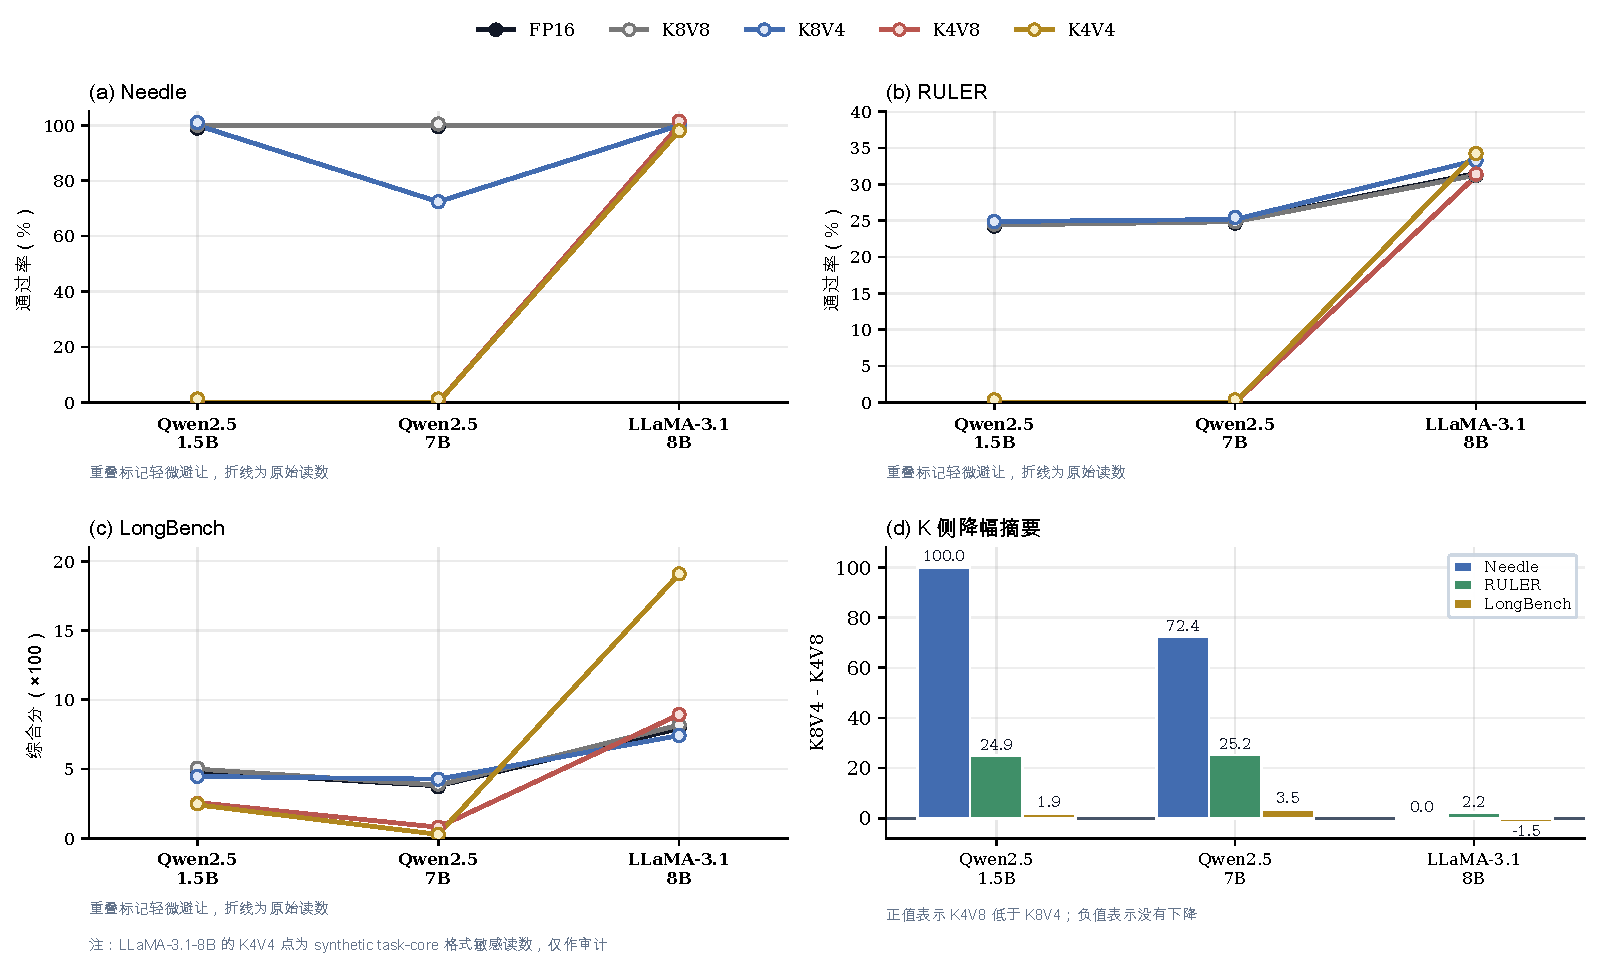
\includegraphics[width=\linewidth]{figures/ch4/fig_ch4_01_kv_ruler32.pdf}
  \caption{K/V 角色敏感性的跨指标诊断图。子图（a）--（c）分别在 Needle、RULER 与 LongBench-style 指标上比较主要位宽布局；横轴为模型，折线表示不同位宽布局的原始分数。为避免完全重叠，部分标记做微小纵向避让，但折线仍连接原始读数。子图（d）汇总 \texttt{K4V8} 相对 \texttt{K8V4} 的下降幅度。Qwen 系列在 \texttt{K4V8}/\texttt{K4V4} 下出现稳定 cliff，而 LLaMA-3.1-8B 不呈现同强度坍塌，因此该现象应理解为受架构调制的 Key-side low-bit 敏感性，而不是所有模型同强度规律。}
  \label{fig:ch4-kv-ruler32}
  \label{fig:kv-ablation-summary-ruler}
\end{figure}

图~\ref{fig:ch4-kv-ruler32} 将 Needle、RULER 与 LongBench-style 放到同一位宽布局矩阵中。Qwen2.5-1.5B 与 Qwen2.5-7B 的共同模式是：\texttt{K8V8} 与 \texttt{K8V4} 大体保持可用，而 \texttt{K4V8} 和 \texttt{K4V4} 在 Needle 与 RULER 上直接跌入 cliff，LongBench-style 也同步下降。LLaMA-3.1-8B 则不表现出同强度 cliff：\texttt{K4V8} 在三类指标上仍接近高精度路径，\texttt{K4V4} 在 Needle 与 RULER 上也未出现同幅度坍塌；其 LongBench-style 高读数作为 synthetic task-core 的格式敏感结果保留在图中，但不用于支持“\texttt{K4V4} 优于 \texttt{FP16}”这一判断。由此，本图支持的结论不是“所有模型都会同样 Key 崩”，而是：4bit Key 扰动在 Qwen 系列上会稳定触发行为崩塌，但其强度受到模型族、规模与 $H_{kv}$ 等架构因素调制。

\begin{figure}[t]
  \centering
  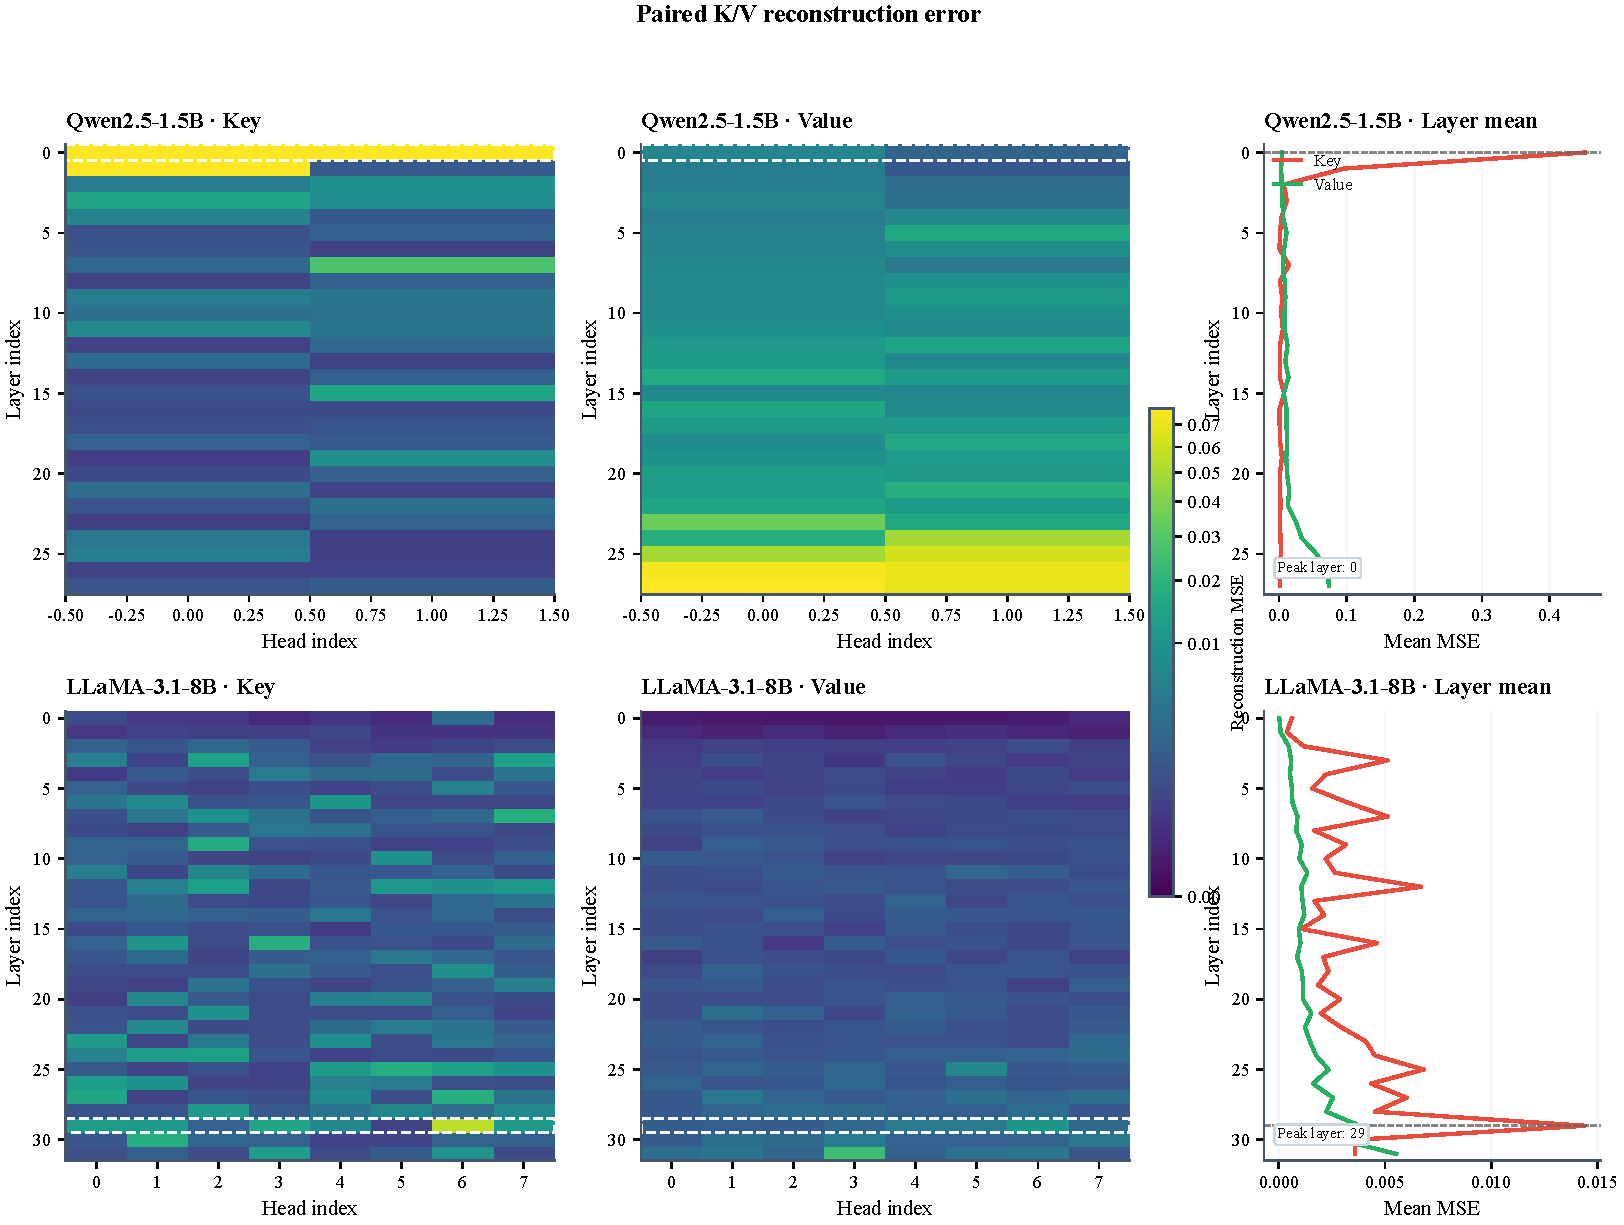
\includegraphics[width=\linewidth]{figures/ch4/fig_ch4_02_kv_error_heatmap.pdf}
  \caption{Qwen2.5-1.5B 与 LLaMA-3.1-8B 的配对 K/V 重建误差热力图（MixedKV，\texttt{K@INT8+V@INT4}，32K 上下文）。上排为 Qwen2.5-1.5B，下排为 LLaMA-3.1-8B；左两列分别为 Key 与 Value 的逐层逐头重建误差，右列为逐层平均误差曲线。统一色标显示：相较于 Qwen2.5-1.5B，LLaMA-3.1-8B 的高误差层段更集中、整体误差更低，与其更强的噪声稀释能力一致。}
  \label{fig:ch4-kv-error-heatmap}
\end{figure}

图~\ref{fig:ch4-kv-error-heatmap} 从误差结构侧补充了这种架构依附性。配对热力图显示，在 \texttt{MixedKV} 配置下，Qwen2.5-1.5B 的高误差层段更早、更分散，而 LLaMA-3.1-8B 的误差峰值则更集中于后部层段，整体量级也更低。这张图不是 attention-KL 主指标的替代物，但它支持了与表~\ref{tab:ch4-kv-multitask} 同方向的解释：在更高 $H_{kv}$ 与更平滑的架构条件下，Key 量化噪声更不容易被放大成检索崩塌。

最后，再用一条补充性扩展把这一结论从小模型与中等规模模型延伸到更大模型。在 Qwen2.5-14B 上，保持 Key 为高精度的 \texttt{K16V4} 可将 PPL 从 full \texttt{INT4} 的 5.040 恢复到 4.709，即恢复约 93\% 的退化；相对地，保持 Value 为高精度的 \texttt{K4V16} 仅能恢复到 4.813，恢复率约 64\%。这表明在当前 14B 的补充对比中，保持 Key 为高精度能够带来更大的恢复幅度。至此，本节可以把诊断结论压成一句设计启示：在本文考察的 low-bit 场景中，真正首先触发行为崩塌的是 Key 精度下降；而 \texttt{MixedKV} 的恢复则表明，低比特路径的首要动作不是继续平均压缩 K/V，而是优先保护 Key，并在此基础上升级量化格式。

\subsection{INT4-RoleAlign 与 KIVI-style 的跨模型对比}
\label{subsec:ch4-rolealign-kivi}
\label{subsec:exp-int4-cross-model}
\label{sec:exp-rolealign}

如果第~\ref{subsec:ch4-kv-diagnosis}~节的结论成立，那么下一步就不应再在对称 \texttt{INT4} 的参数空间中继续调参，而应进入 role-aware 非对称格式空间。在这一空间内，本文采用的 \texttt{INT4-RoleAlign} 与 \texttt{KIVI-style} 共享相同的缓存格式，即 \texttt{per-channel K + per-token V}；因此，本小节比较的是同一量化格式下两种校准实例化方式。二者在设计层面的差异已在第三章第~\ref{subsec:ch3-rolealign-vs-kivi}~节中说明，这里不再重复放置设计差异表，而是集中报告同格式条件下的经验结果，并在表注中区分完整配对比较与仅用于界定适用范围的行。

\begin{table}[t]
  \centering
  \caption{INT4-RoleAlign 与 KIVI-style 的跨模型主对比}
  \label{tab:ch4-rolealign-kivi}
  \label{tab:t2-int4-kivi}
  {%
  \footnotesize
  \setlength{\tabcolsep}{4pt}
  \renewcommand{\arraystretch}{1.05}
  \begin{tabular}{lccccccc}
    \toprule
    模型 & $H_{kv}$ & FP16 PPL & KIVI-style PPL & RoleAlign PPL & $\Delta$PPL & KIVI Needle & RoleAlign Needle \\
    \midrule
    Qwen2.5-1.5B & 2 & 9.31 & 10.43 & 10.58 & +0.15 & 100/100\% & 100/100\% \\
    Qwen2.5-7B   & 4 & 7.14 & 7.53  & 7.58  & +0.05 & 100/100\% & 100/100\% \\
    LLaMA-3.1-8B & 8 & 6.73 & 6.90  & 6.90  & +0.00 & 100/100\% & 100/100\% \\
    Qwen2.5-14B  & 8 & 4.68 & --    & 5.04  & --    & --         & 100/100\% \\
    \bottomrule
  \end{tabular}

  \vspace{0.35em}
  \begin{minipage}{0.94\linewidth}
    \footnotesize
    注：两者共享 \texttt{per-channel K + per-token V} 非对称格式，唯一差异是校准理念：\texttt{RoleAlign} 采用离线 role-aware calibration，其中 K-path 以 attention-distribution KL 为主代理，并在离线搜索纪律下确定参数，V-path 由独立输出扰动代理主导；\texttt{KIVI-style} 使用运行时 \texttt{absmax/min}。Needle 列中的“100/100”表示 \texttt{Needle-single-retrieval} 与 \texttt{MK-NIAH-2} 两类检索同时恢复到 100\%。Qwen2.5-1.5B、Qwen2.5-7B 与 LLaMA-3.1-8B 构成当前正文中的完整配对对比；Qwen2.5-14B 当前仅提供 RoleAlign 结果，因此该行主要用于界定比较范围，而不参与配对差异判断。为保持与现有结果资产的一致性，1.5B 行采用当前主协议下的重跑结果，7B/8B/14B 行采用同格式、同指标定义下的既有对比结果。
  \end{minipage}
  }
\end{table}

表~\ref{tab:ch4-rolealign-kivi} 显示，在共享非对称格式的前提下，\texttt{INT4-RoleAlign} 与 \texttt{KIVI-style} 的经验差距并不是一边倒式的大缺口。在当前可直接配对的 1.5B、7B 与 8B 三个模型上，RoleAlign 相对 KIVI-style 的 PPL 差距分别为 $+0.15$、$+0.05$ 与 $+0.00$；Needle 则在三者上都恢复到 100/100\%。14B 的 RoleAlign 行只用于说明该格式在更大模型上的当前覆盖范围，不参与差异判断。这一结果首先说明：\textbf{决定低比特检索恢复的关键首先是角色感知非对称格式本身。} 一旦从对称 per-group 升级到 \texttt{per-channel K + per-token V}，低比特路径就已经从“完全崩塌”转回“可用状态”。在此基础上，校准理念的差异更多体现在实例化方式，而不是大幅拉开质量缺口。

离线行为引导校准的独立价值主要体现在组织方式而非一边倒的经验差距。当前证据支持的更稳解释是：在同格式条件下，\texttt{RoleAlign} 的优势不在于把 \texttt{KIVI-style} 远远甩开，而在于它把低比特路径组织成了一条\textbf{可固化、可审计、可扩展}的实例化路径。\texttt{KIVI-style} 依赖运行时 \texttt{absmax/min} 重算 scale，\texttt{RoleAlign} 则将 K-path 与 V-path 的分路校准结果固化为离线校准结果；也正因为如此，\texttt{RoleAlign} 才能自然延伸到后续的行为引导分配器，而不是停留在一个只做运行时统计的缓存格式基线上。本小节支持的是“格式是一阶、离线校准是二阶组织增益”的当前判断。

至此，低比特恢复问题已经得到回答：第~\ref{subsec:ch4-int4-cliff}~节说明行为引导原则在对称 \texttt{INT4} 上首先遭遇架构依附性的阶跃失效；第~\ref{subsec:ch4-kv-diagnosis}~节进一步表明，该失效主要由 Key 侧精度下降触发，而 \texttt{MixedKV} 的恢复指向“Key 优先保护”与角色感知格式升级；最后，本小节说明在共享非对称格式的公平设置下，\texttt{INT4-RoleAlign} 可以把这一路径恢复为一个可审计、可扩展的低比特实例。接下来的问题，不再是低比特路径能否被恢复，而是恢复后的行为敏感度画像能否进一步支撑跨模型预算分配，并读出稳定的策略适用区间结构。

\section{跨模型预算分配与策略适用区间图谱}
\label{sec:ch4-rq3}
\label{sec:exp-cross-model}
\label{sec:exp-per-model}

第~\ref{sec:ch4-rq2} 节已经确认，低比特路径可以在角色感知非对称格式下被恢复。本节进一步回答跨模型预算分配问题：由行为引导校准产出的敏感度画像，是否能够支撑跨模型预算分配，并揭示稳定的策略适用区间结构。本节的目标不是寻找一个跨模型的单一普适最优策略，而是把分配器结果从若干跑分表提升为一张可命名的适用区间图谱。

为避免将 allocator 结果误读为单一策略排名，本节首先在同量级 INT4 预算带内给出跨模型主表，再通过四个典型剖面概括不同模型上的结构落点。这里所谓“策略适用区间”，指的是在给定模型族、规模与任务组合下，某类 allocator 策略更容易落在该模型的高性能区间，而不是在严格同预算条件下已经被形式化证明更优。

\subsection{同量级预算下的跨模型主表}
\label{subsec:ch4-regime-main}

本节先明确比较口径。表~\ref{tab:ch4-regime-main} 报告的是同量级 INT4 预算带内的结构读数，而不是严格同显存的 $\pm 3\%$ 对照。当前各 allocator 策略的平均位宽大致落在 $4.5\text{--}5.0$ bit 带内，而 uniform \texttt{INT4} 对应 $\bar b = 4.0$ bit，因此这里的主要作用，是回答“在同一数量级预算内，不同分配风格会在不同模型上落到哪里”，而不是回答“在严格同预算下谁被形式化证明更优”。这一边界同时也是本节与未来严格同预算比较的分界线。

\begin{table}[t]
  \centering
  \caption{同量级 INT4 预算带内的跨模型主表}
  \label{tab:ch4-regime-main}
  \label{tab:t3-cross-model-main}
  {%
  \footnotesize
  \setlength{\tabcolsep}{4pt}
  \renewcommand{\arraystretch}{1.05}
  \begin{tabular}{llcccc}
    \toprule
    模型 & 任务/汇总 & Uniform INT4 & BA-k & Heuristic-k & BA-AutoK \\
    \midrule
    \multirow{4}{*}{Qwen2.5-3B ($H_{kv}=2$)}
      & NarrativeQA (F1)    & 4.33 & \textbf{7.17} & 3.08 & 6.48 \\
      & HotpotQA (F1)       & 2.38 & 4.73 & 1.39 & \textbf{4.89} \\
      & GovReport (Rouge-L) & 5.77 & 8.81 & 5.96 & \textbf{8.90} \\
      & Mean                & 4.16 & \textbf{6.90} & 3.48 & 6.75 \\
    \midrule
    \multirow{4}{*}{LLaMA-3.1-8B ($H_{kv}=8$)}
      & NarrativeQA (F1)    & 10.24 & \textbf{11.14} & 10.47 & 10.74 \\
      & HotpotQA (F1)       & 6.73  & \textbf{7.88}  & 5.68  & 7.57 \\
      & GovReport (Rouge-L) & 9.24  & 9.54 & 9.47 & \textbf{9.75} \\
      & Mean                & 8.74  & \textbf{9.52} & 8.54 & 9.35 \\
    \midrule
    \multirow{4}{*}{Qwen2.5-14B ($H_{kv}=8$)}
      & NarrativeQA (F1)    & \textbf{7.05} & 6.67 & 6.83 & 6.80 \\
      & HotpotQA (F1)       & \textbf{5.57} & 5.49 & 5.40 & 5.39 \\
      & GovReport (Rouge-L) & 9.09 & 8.95 & 9.03 & \textbf{9.27} \\
      & Mean                & \textbf{7.23} & 7.04 & 7.09 & 7.15 \\
    \midrule
    \multirow{4}{*}{Mistral-7B-v0.3 ($H_{kv}=8$)}
      & NarrativeQA (F1)    & 15.55 & 15.71 & \textbf{17.11} & 16.26 \\
      & HotpotQA (F1)       & 17.81 & 17.78 & 17.84 & \textbf{19.08} \\
      & GovReport (Rouge-L) & 8.70  & 8.66  & 8.86 & \textbf{8.96} \\
      & Mean                & 14.02 & 14.05 & 14.60 & \textbf{14.76} \\
    \bottomrule
  \end{tabular}

  \vspace{0.35em}
  \begin{minipage}{0.94\linewidth}
    \footnotesize
    注：本表报告的是同量级 INT4 预算带内的跨模型读数，而不是严格同预算比较。各模型的 best-$k$ 动态选择为：Qwen2.5-3B 用 $k=1$，LLaMA-3.1-8B 用 $k=11$，Qwen2.5-14B 用 $k=7$，Mistral-7B 用 $k=3$；AutoK 的覆盖阈值在 14B 上为 90\%，其余模型为 80\%。Uniform 指所有层 K/V 统一采用 INT4；BA-k 指 behavior-guided allocator 保护 top-$k$ 高敏感层；Heuristic-k 指等距位置启发式保护；BA-AutoK 指根据覆盖率准则自动确定保护层数的 behavior-guided allocator。
  \end{minipage}
  }
\end{table}

表~\ref{tab:ch4-regime-main} 的核心信息不是“哪一列整体最高”，而是四个模型的最佳策略家族并不一致：Qwen2.5-3B 的三任务均值最优落在 BA-k1，LLaMA-3.1-8B 的三任务均值最优落在 BA-k11，Qwen2.5-14B 的最高均值落在 Uniform，而 Mistral-7B 的三任务均值最优则落在 BA-AutoK。这些差异并不能仅凭与敏感度画像的对应关系单独成立；它们首先需要与图~\ref{fig:ch4-autok-protection} 中的保护层结构相互印证，而图~\ref{fig:ch4-regime-heatmap} 则把这种异质性整理为后续四个模型剖面的阅读路线图。

\begin{figure}[t]
  \centering
  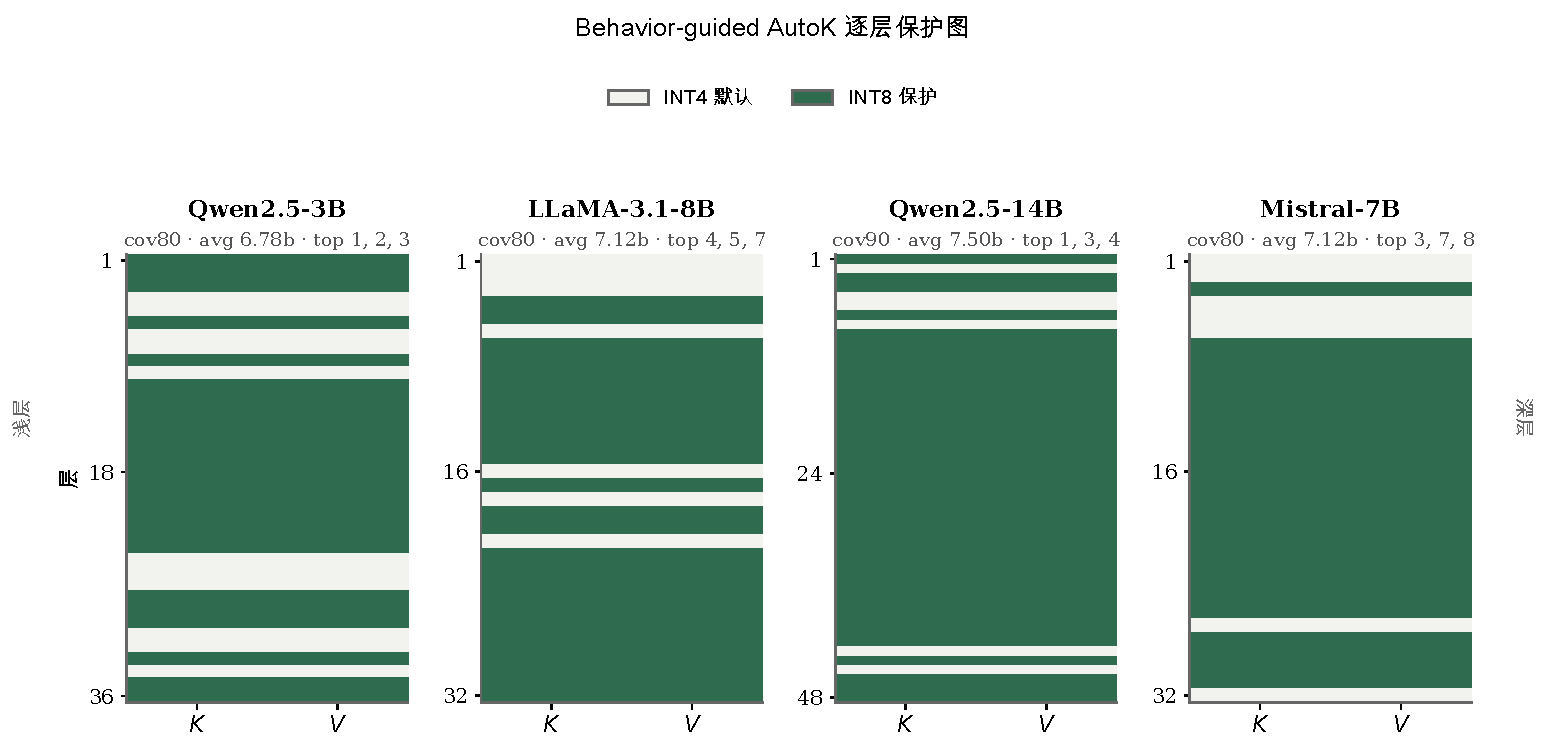
\includegraphics[width=\linewidth]{figures/ch4/fig_ch4_03_autok_protection_map.pdf}
  \caption{Behavior-guided AutoK 的逐层保护决策。四个子图分别对应 Qwen2.5-3B、LLaMA-3.1-8B、Qwen2.5-14B 与 Mistral-7B，展示同一 coverage 规则下各模型的保护层结构。该图将跨模型主表背后的 sensitivity shape 直接可视化。}
  \label{fig:ch4-autok-protection}
  \label{fig:sensitivity-heatmap}
\end{figure}

图~\ref{fig:ch4-autok-protection} 把这种结构差异直接可视化。Qwen2.5-3B 的保护层明显前移并集中于最早层，说明其 sensitivity profile 呈现典型的 early-layer bottleneck；LLaMA-3.1-8B 与 Mistral-7B 则呈现中层簇集，说明在中等规模与特定家族上，真正关键的层已经不是单一首层，而是一簇相邻的高敏感层；Qwen2.5-14B 则近乎铺满全深度，表现为广泛铺展的 profile，说明大模型的行为敏感度已经显著弥散化。于是，“不同模型最优项不同”不再只是表格现象，而与 sensitivity structure 的差异相互印证。

\begin{figure}[t]
  \centering
  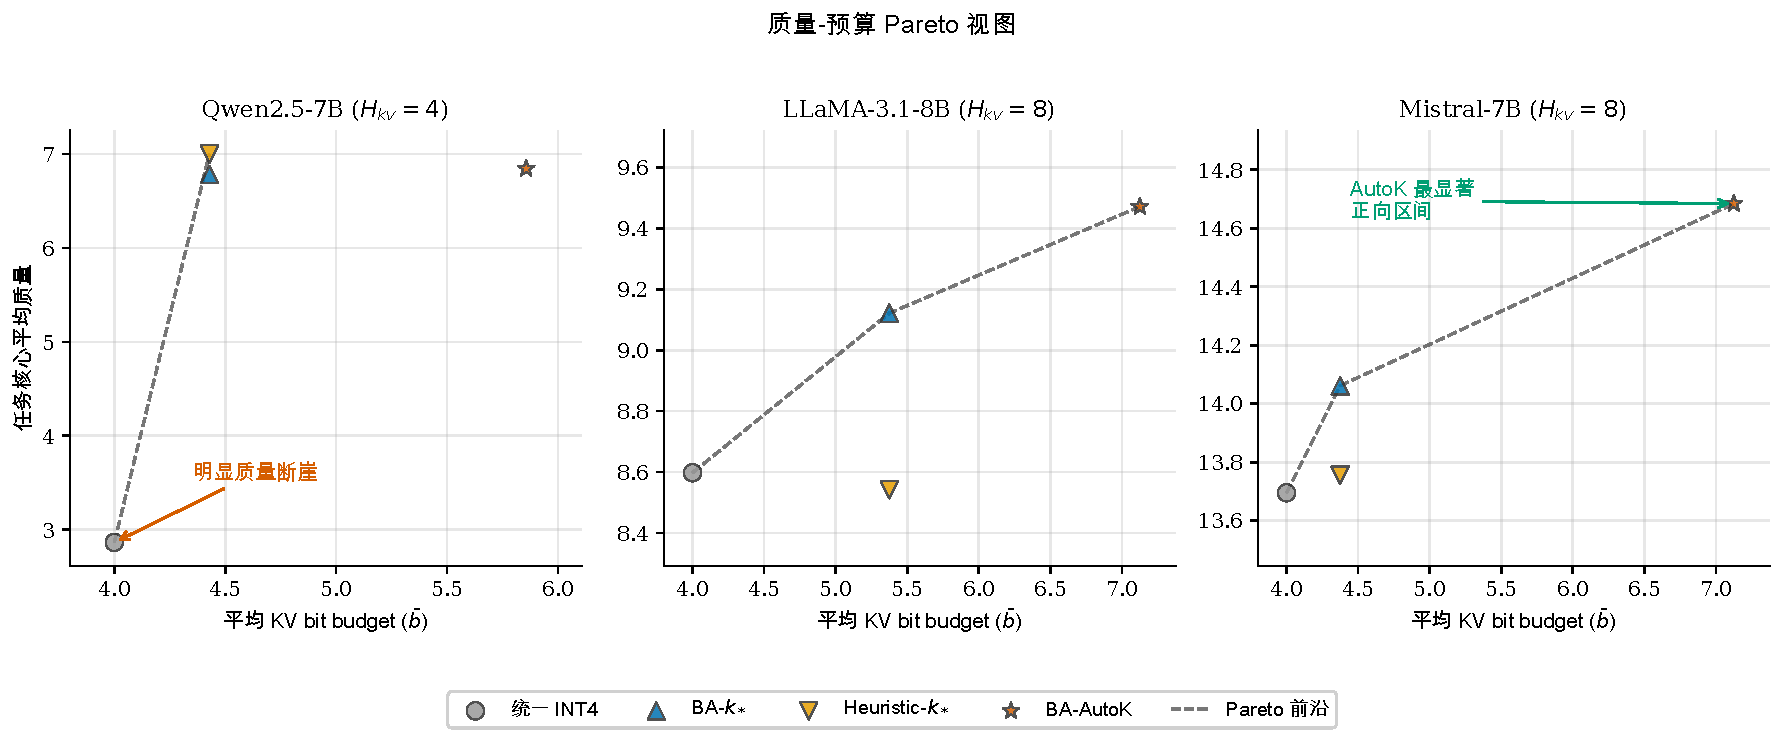
\includegraphics[width=\linewidth]{figures/ch4/fig_ch4_04_pareto_budget_quality.pdf}
  \caption{质量-预算 Pareto 视图。三个子图分别对应 Qwen2.5-7B、LLaMA-3.1-8B 与 Mistral-7B；横轴为平均 KV bit budget，纵轴为任务核心平均质量。该图用于可视化同量级 INT4 预算带下不同策略家族的局部几何关系，而不是严格的同预算比较。}
  \label{fig:ch4-pareto}
  \label{fig:t7-pareto}
\end{figure}

\begin{figure}[t]
  \centering
  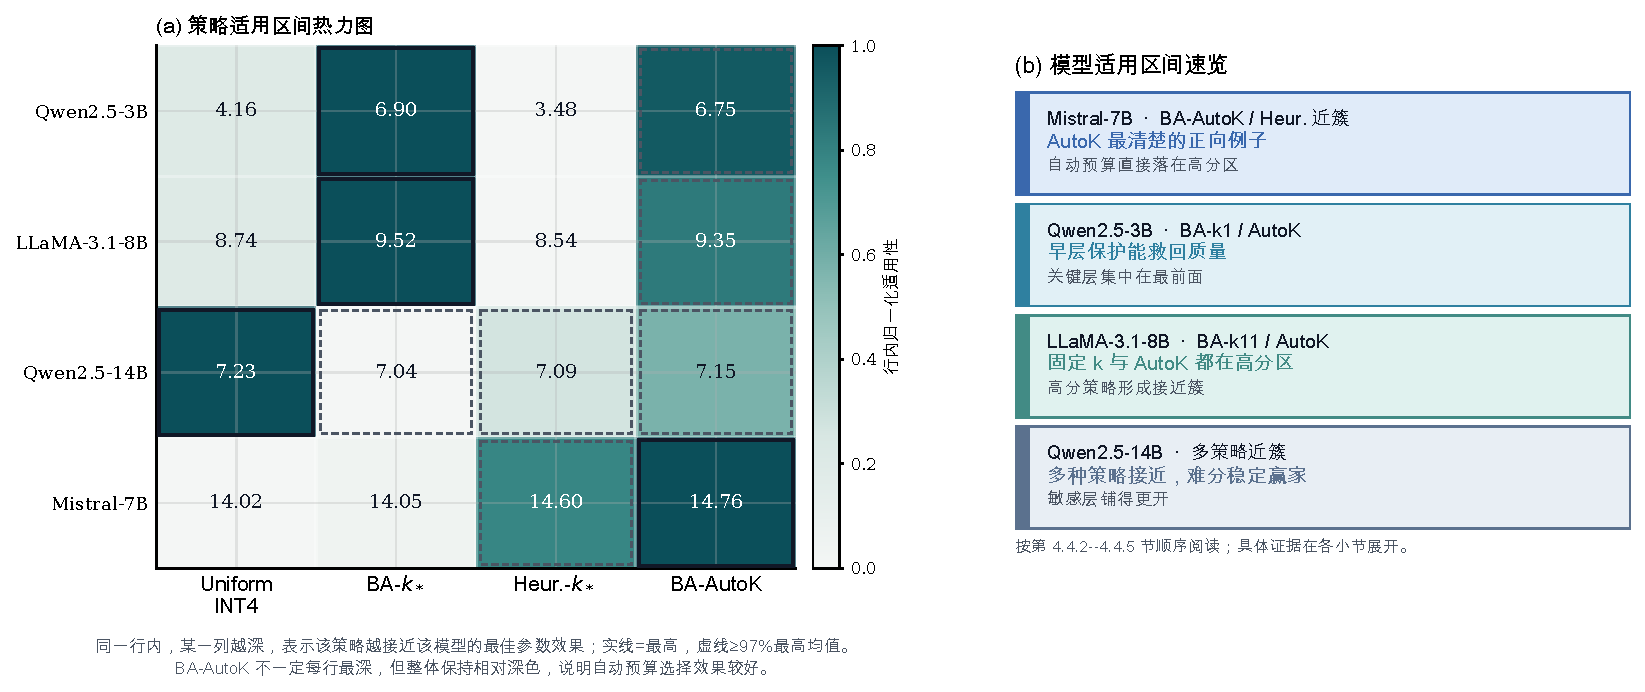
\includegraphics[width=\linewidth]{figures/ch4/fig_ch4_05_regime_heatmap.pdf}
  \caption{跨模型策略适用区间与模型适用区间速览。左图展示各模型在四类策略家族下的任务核心平均质量；同一模型所在行内，某一列颜色越深表示该策略越接近该模型的高性能区间，但颜色不表示跨模型绝对质量可比。BA-AutoK 列虽然并非每行最深，但整体处于相对深色区间，因此可视为效果较好的自动预算候选。实线边框标出每行最高落点，虚线边框标出达到该行最高三任务均值 $97\%$ 以上的近簇。右图按后文模型分析顺序列出四类待展开结构类型，作为第 4.4.2--4.4.5 节的阅读路线图。}
  \label{fig:ch4-regime-heatmap}
\end{figure}

图~\ref{fig:ch4-pareto} 与图~\ref{fig:ch4-regime-heatmap} 进一步把主表读成适用区间，而不是简单排名。Pareto 图说明同量级预算带内确实存在清晰的质量--预算局部几何：Mistral-7B 上 AutoK 区域最为突出，LLaMA-3.1-8B 上几种高性能策略形成近 Pareto 的局部簇；Qwen2.5-7B 的补充结果只作为 uniform policy 质量断崖的旁证，不进入后文四个模型剖面节。合并后的适用区间图则承担两层作用：左图把四模型压缩成“每行一个高性能落点”的速览图，右图按 Mistral-7B、Qwen2.5-3B、LLaMA-3.1-8B 与 Qwen2.5-14B 的后文顺序提示四个待展开结构类型，而不是在本小节完成证明。值得注意的是，position-based heuristic 在多个区间内与 behavior-guided 选中集合发生重合；这一强基线现象的结构性含义，将在第 4.6.3 节中进一步讨论。

\subsection{Mistral-7B：AutoK 的单模型支持证据}
\label{subsec:ch4-profile-mistral}
\label{subsec:exp-per-model-mistral}

Mistral-7B 被单独列出，是因为它提供了当前最清晰的 AutoK 单模型支持证据。该剖面的价值不在于证明“AutoK 普适最优”，而在于回答一个更窄也更重要的问题：当敏感度画像本身具有可压缩的中层簇集结构时，覆盖度预算建议能否读出层间结构。

\begin{table}[t]
  \centering
  \caption{典型剖面表 A：Mistral-7B 与 Qwen2.5-3B}
  \label{tab:ch4-profile-a}
  \label{tab:t4-mistral-autok}
  \label{tab:t5-3b-early-layer}
  {%
  \footnotesize
  \setlength{\tabcolsep}{4pt}
  \renewcommand{\arraystretch}{1.05}
  \begin{tabular}{lcccccc}
    \toprule
    \multicolumn{7}{l}{\textbf{Panel A. Mistral-7B：AutoK 的单模型支持证据}} \\
    \midrule
    任务 & Uniform & BA-k3 & Heuristic-k3 & \makecell[c]{BA-AutoK\\(80\%)} & 最优项 & 备注 \\
    \midrule
    NarrativeQA (F1)    & 15.55 & 15.71 & \textbf{17.11} & 16.26 & Heur-k3 & \\
    HotpotQA (F1)       & 17.81 & 17.78 & 17.84 & \textbf{19.08} & AutoK & \\
    GovReport (Rouge-L) & 8.70  & 8.66  & 8.86 & \textbf{8.96}  & AutoK & \\
    DuReader (Rouge-L)  & 7.35  & 8.64  & 7.97 & \textbf{11.62} & AutoK & 增益最大 \\
    LCC (EditSim)       & 21.38 & \textbf{22.10} & 20.30 & 19.77 & BA-k3 & \\
    Mean                & 14.16 & 14.58 & 14.42 & \textbf{15.14} & AutoK & 5-task mean \\
    \midrule
    \multicolumn{7}{l}{\textbf{Panel B. Qwen2.5-3B：早层保护有效区间}} \\
    \midrule
    任务 & Uniform & BA-k1 & Heuristic-k1 & \makecell[c]{BA-AutoK\\(80\%)} & Quality $\Delta$ & 备注 \\
    \midrule
    NarrativeQA (F1)    & 4.33 & \textbf{7.17} & 3.08 & 6.48 & +4.09 & 提升 \\
    HotpotQA (F1)       & 2.38 & 4.73 & 1.39 & \textbf{4.89} & +3.33 & 提升 \\
    GovReport (Rouge-L) & 5.77 & 8.81 & 5.96 & \textbf{8.90} & +2.85 & 提升 \\
    Mean                & 4.16 & \textbf{6.90} & 3.48 & 6.75 & +3.42 & 差距最大 \\
    \bottomrule
  \end{tabular}

  \vspace{0.35em}
  \begin{minipage}{0.94\linewidth}
    \footnotesize
    注：Panel A 来自 Mistral-7B-v0.3 的 5-task 扩展剖面；Panel B 来自 Qwen2.5-3B 的 3-task task-core 剖面。Mistral 的 AutoK 覆盖阈值为 80\%；Qwen2.5-3B 的 behavior-guided best-$k$ 为 $k=1$。本表由第 4.4.2 节与第 4.4.3 节共用，并以双剖面块形式组织。
  \end{minipage}
  }
\end{table}

表~\ref{tab:ch4-profile-a} 的 Panel A 显示，BA-AutoK 在 Mistral-7B 的五个任务中有三个任务给出最高读数，并取得最高平均值。最明显的差异来自 DuReader：BA-AutoK 达到 11.62，而 Heuristic-k3 为 7.97，差距达到 3.6 分；同时，它在 HotpotQA 与 GovReport 上也给出最优读数。由于这些增益分散在多个任务上，而不是由单一异常任务造成，因此它们支持一种基于覆盖率的正向解释，而不只是单个数据集上的偶然波动。

这一优势与图~\ref{fig:ch4-autok-protection} 中的敏感度画像是一致的。Mistral-7B 的重点保护层落在中前层簇集，且 80\% 覆盖阈值选出的保护范围与这种簇集结构相吻合，因此 AutoK 在这里并非偶然获得更好的预算，而是与覆盖率预算建议器所捕捉到的层间结构保持一致。于是，Mistral-7B 在本文中承担的不是“AutoK 跨设置最优”的证明，而是“当画像具有可压缩簇集结构时，覆盖率预算建议器可以给出清晰正向信号”的单模型实例。

\subsection{Qwen2.5-3B：早层保护有效区间}
\label{subsec:ch4-profile-qwen3b}
\label{subsec:exp-per-model-3b}

Qwen2.5-3B 则承担了全文最清晰的行为引导策略与位置启发式差距剖面。它之所以单列，不是因为总体分数最高，而是因为它揭示了一类更窄但更重要的适用区间：当行为敏感度高度集中于最早几层时，保护正确的第一层会产生质量提升，而位置启发式若把预算投向“看起来更居中”的层，可能难以覆盖关键瓶颈位置。

表~\ref{tab:ch4-profile-a} 的 Panel B 给出了这一点的主要数字支撑。对 BA-k1 与 Heuristic-k1 的直接比较表明，BA-k1 在 NarrativeQA 上高出 4.09 分，在 HotpotQA 上高出 3.33 分，在 GovReport 上高出 2.85 分，平均差距达到 3.42 分。这里最关键的不是增益的绝对量，而是增益的语义：这些差距对应于从低质量区间进入可用区间，因此应被读作早层保护带来的质量提升。

这一恢复性收益与图~\ref{fig:ch4-autok-protection} 的 3B 结构读数一致。Qwen2.5-3B 的敏感度画像明显前移，top protected layers 集中在最早层；BA-k1 保护的是 layer 0，而 Heuristic-k1 的单层保护则落在中层，因而偏离瓶颈层。3B 并不是在证明“小模型总该用 BA-k1”，而是在定义一种更精确的适用区间：当行为敏感度在最早几层高度集中时，位置启发式可能偏离关键层，而行为引导保护可以产生恢复性收益。

\subsection{LLaMA-3.1-8B：中等规模共识区间}
\label{subsec:ch4-profile-llama8b}

LLaMA-3.1-8B 是当前主线中的一个重要模型案例。跨模型主表已经显示出足够清晰的结构信号：最佳平均值落在 BA-k11，同时 BA-AutoK 与其它高性能策略距离并不远。因此，本节将这行结果展开为一个可单独讨论的结构区间。

\begin{table}[t]
  \centering
  \caption{典型剖面表 B：LLaMA-3.1-8B 与 Qwen2.5-14B}
  \label{tab:ch4-profile-b}
  \label{tab:t6-14b-toptier}
  {%
  \footnotesize
  \setlength{\tabcolsep}{4pt}
  \renewcommand{\arraystretch}{1.05}
  \begin{tabular}{lcccccc}
    \toprule
    \multicolumn{7}{l}{\textbf{Panel A. LLaMA-3.1-8B：中等规模共识区间}} \\
    \midrule
    任务 & Uniform & BA-k11 & Heuristic-k11 & \makecell[c]{BA-AutoK\\(80\%)} & 最优项 & 备注 \\
    \midrule
    NarrativeQA (F1)    & 10.24 & \textbf{11.14} & 10.47 & 10.74 & BA-k11 & \\
    HotpotQA (F1)       & 6.73  & \textbf{7.88}  & 5.68  & 7.57  & BA-k11 & \\
    GovReport (Rouge-L) & 9.24  & 9.54 & 9.47 & \textbf{9.75} & AutoK & \\
    Mean                & 8.74  & \textbf{9.52} & 8.54 & 9.35 & BA-k11 & 共识高性能区间 \\
    \midrule
    \multicolumn{7}{l}{\textbf{Panel B. Qwen2.5-14B：高性能簇共存而无稳定最优}} \\
    \midrule
    任务 & Uniform & BA-k7 & Heuristic-k7 & \makecell[c]{BA-AutoK\\(90\%)} & $gap_{\mathrm{rel}}$ & 备注 \\
    \midrule
    NarrativeQA (F1)    & \textbf{7.05} & 6.67 & 6.83 & 6.80 & 3.55\% & top-3 聚簇 \\
    HotpotQA (F1)       & \textbf{5.57} & 5.49 & 5.40 & 5.39 & 3.05\% & top-3 聚簇 \\
    GovReport (Rouge-L) & 9.09 & 8.95 & 9.03 & \textbf{9.27} & 2.59\% & top-3 聚簇 \\
    Mean                & \textbf{7.23} & 7.04 & 7.09 & 7.15 & 3.06\% & max $\approx$ 3.5\% \\
    \bottomrule
  \end{tabular}

  \vspace{0.35em}
  \begin{minipage}{0.94\linewidth}
    \footnotesize
    注：Panel A 展示 LLaMA-3.1-8B 的中等规模共识区间；Panel B 展示 Qwen2.5-14B 的高性能策略簇。Qwen2.5-14B 的 \mbox{$gap_{\mathrm{rel}}(t)=(top1(t)-top3(t))/top1(t)$} 最大约 3.5\%，平均约 3.0\%。在当前统计功效下，14B 的高性能策略更适合解释为近似不可分辨的策略簇，而不是稳定单一最优。
  \end{minipage}
  }
\end{table}

表~\ref{tab:ch4-profile-b} 的 Panel A 表明，LLaMA-3.1-8B 的确存在一个较明确的 BA-k11 结构落点：NarrativeQA 与 HotpotQA 上 BA-k11 都给出最优读数，GovReport 上则由 BA-AutoK 略占优势，最终平均值由 BA-k11 取得最优。这里最值得强调的不是单点策略相对其它策略形成绝对优势，而是它与 BA-AutoK 之间的差距非常有限；再结合图~\ref{fig:ch4-pareto} 中近 Pareto 的局部几何关系，更合理的读法是：LLaMA-3.1-8B 所代表的，是一个 \emph{共识高性能区间}，而不是单点独占。

这一命名与其敏感度画像形状也是一致的。与 Qwen2.5-3B 的尖锐前层集中不同，LLaMA-3.1-8B 的最佳保护范围已经扩展到更广的中层簇集，best-$k=11$ 本身就意味着“单点保护”不再是合理抽象；但与此同时，它又不像 Qwen2.5-14B 那样弥散到几乎全深度广泛铺展。因此，LLaMA-3.1-8B 最适合被命名为 \textbf{中等规模共识区间}：存在一个相对稳定的 BA-k 结构落点，但其它高性能策略并未远离。它在本文中还承担一个更克制的对照角色：由于其 $H_{kv}=8$ 设置与较平滑的分配器响应同时出现，我们可以把它当作 GQA 架构稳健性的补充剖面，但不能把它升级为“更高 $H_{kv}$ 必然导向更优策略”的强结论。

\subsection{Qwen2.5-14B：高性能簇共存而无稳定最优}
\label{subsec:ch4-profile-qwen14b}
\label{subsec:exp-per-model-14b}

Qwen2.5-14B 提供的是这张适用区间图谱中的边界剖面：并非每个模型都会给出清晰最优项。它在跨模型主表中的最高均值落在 Uniform，但这一读数如果被直接概括为“Uniform 最优”，就会弱化 14B 的结构形状。对于这个模型，更关键的事实不是某一策略在平均分上略高，而是几类高性能策略彼此接近，以至于在当前证据下更适合被读成近似持平的策略簇。

表~\ref{tab:ch4-profile-b} 的 Panel B 直接支持这一点。三个任务上四类策略的数值都非常接近，按照 $gap_{\mathrm{rel}}(t)=(top1(t)-top3(t))/top1(t)$ 的定义，NarrativeQA、HotpotQA 与 GovReport 的 top-3 相对 top-1 gap 分别约为 3.55\%、3.05\% 与 2.59\%，平均值约为 3.06\%。这意味着 14B 的 top-3 策略全部位于 top-1 的 3.5\% 相对距离内。基于这些相对差距，更稳的解释不是“Uniform 真正最优”，而是：\textbf{14B 当前呈现出一个高性能策略彼此接近的簇，而不是稳定单一最优。}

这种近似持平的格局与图~\ref{fig:ch4-autok-protection} 的广泛铺展画像是一致的。Qwen2.5-14B 的敏感度画像已经近乎铺满全深度，AutoK 在 48 层中标出 42 个受保护层，说明它不是由少数关键层决定一切的模型。正因为画像本身已经高度弥散，分配器在当前预算区间中的选择顺序只会带来有限边际影响。于是，14B 给这张适用区间图谱的不是一个正面最优项，而是一条更稳的结构结论：\textbf{高性能簇共存而无稳定最优。}

回到图~\ref{fig:ch4-regime-heatmap} 的右图，第 4.4 节的四个模型剖面最终对应四类结构类型：Mistral-7B 提供 AutoK 的单模型支持证据，Qwen2.5-3B 是早层保护有效区间，LLaMA-3.1-8B 是中等规模共识区间，Qwen2.5-14B 则是高性能簇共存而无稳定最优。它们共同构成一张按模型族、规模与任务共同决定的适用区间图谱，而不是“哪个策略全局最好”的排行榜。至此，跨模型预算分配问题已经得到回答：行为敏感度画像不只是校准层的副产物，它还能在同量级预算带内支撑跨模型预算分配，并读出稳定而可命名的结构落点。下一节将不再继续讨论质量适用区间，而转向这些路径在真实推理系统中的时间与显存边界。

\section{部署效率评估}
\label{sec:ch4-deployment}
\label{sec:exp-deployment}

第~\ref{sec:ch4-rq1}--\ref{sec:ch4-rq3} 节已经分别回答了基准保真、low-bit 恢复与跨模型策略图谱。本节转向部署层，考察这些路径在真实推理系统中的时间与显存代价。本节不再重复第三章关于 kernel 设计与离线校准产物的实现细节，而是聚焦一个更务实的问题：\emph{在什么条件下，当前低比特部署路径能够带来部署收益；在什么条件下，其收益会受到限制。}

为此，本节按“入口读数 $\rightarrow$ 长序列放大 $\rightarrow$ 经验边界 $\rightarrow$ 部署建议”的顺序组织。首先，第~\ref{subsec:ch4-tpot-4k}~节给出 4K 序列下的后端路径入口读数，避免把任何后续加速误读为无条件现象；随后，第~\ref{subsec:ch4-tpot-scaling}~节展示长序列下融合路径收益如何随上下文增长而放大；在此基础上，第~\ref{subsec:ch4-crossover}~节将这些单点与单模型结果上升为一条可读出的性能交叉边界；最后，第~\ref{subsec:ch4-kvcache}~节用 \texttt{KV Cache} 显存压缩率与当前硬件约束将系统层结论收束为可执行部署建议。

\subsection{4K 序列下的 TPOT 对比}
\label{subsec:ch4-tpot-4k}

短上下文入口层的读数是部署判断的起点。4K 序列既是常见的部署长度点，也是判断固定 kernel 开销是否已经值得付出的最低长度点。因此，这一小节的目的不是证明融合路径已经普适占优，而是先给出各后端路径在当前硬件与 batch 设定下的入口层读数：哪些模型上 Triton 融合路径仍受固定调度开销影响，哪些模型上它已经开始逼近甚至略微越过参考路径。

\begin{table}[t]
  \centering
  \caption{4K 序列下的 TPOT 对比（生成长度 128，batch size 为 1，NVIDIA H20；单位：ms）}
  \label{tab:ch4-tpot-4k}
  {%
  \footnotesize
  \setlength{\tabcolsep}{4pt}
  \renewcommand{\arraystretch}{1.05}
  \begin{tabular}{lccccccc}
    \toprule
    模型 & $H_{kv}$ & FP16 & \makecell[c]{参考路径\\(INT4)} & KIVI(INT4) & \makecell[c]{Triton 融合路径\\(INT4)} & FlashInfer(INT4) & 最快项 \\
    \midrule
    Qwen2.5-1.5B & 2 & 24.36 & 36.35 & 36.39 & 38.68 & 43.73 & 参考路径 \\
    Qwen2.5-7B   & 4 & 24.82 & 37.61 & 37.41 & 38.76 & 47.07 & KIVI \\
    LLaMA-3.1-8B & 8 & 28.55 & 44.88 & 44.70 & \textbf{44.49} & 51.50 & Triton 融合路径 \\
    Qwen2.5-14B  & 8 & 42.58 & 68.07 & 68.46 & \textbf{67.67} & 85.07 & Triton 融合路径 \\
    \bottomrule
  \end{tabular}

  \vspace{0.35em}
  \begin{minipage}{0.94\linewidth}
    \footnotesize
    注：粗体标注同模型 INT4 后端路径中的最快项。该表作为第 4.5.1 节的入口层对照，不承担显著加速宣称；真正的收益边界需结合后续长序列读数与性能交叉边界共同解释。
  \end{minipage}
  }
\end{table}

表~\ref{tab:ch4-tpot-4k} 给出三类清楚但应被克制解释的现象：
\begin{itemize}[leftmargin=2em,itemsep=2pt,topsep=2pt]
  \item 在 $H_{kv}=2$ 的 Qwen2.5-1.5B 上，Triton 融合路径录得 38.68\,ms，高于参考路径的 36.35\,ms。
  \item 在 $H_{kv}=4$ 的 Qwen2.5-7B 上，Triton 融合路径录得 38.76\,ms，也高于参考路径的 37.61\,ms。
  \item 只有在 $H_{kv}=8$ 的两种模型上，Triton 融合路径才开始成为该模型下最快的 INT4 后端路径。对 LLaMA-3.1-8B 与 Qwen2.5-14B，其 TPOT 分别为 44.49\,ms 与 67.67\,ms。
\end{itemize}
4K 入口层的读数不应被写成“融合路径已经普适占优”；它只是一个前置信号：当 $H_{kv}$ 较小、Grid 规模不足时，Triton 的固定调度开销仍然可见，而在 $H_{kv}=8$ 上，融合路径已开始逼近甚至轻微越过参考路径，但清晰优势仍要到长序列下才能被放大。

\subsection{长序列 TPOT 扩展规律}
\label{subsec:ch4-tpot-scaling}

如果 4K 入口层只是一个“优势可能开始出现”的信号，那么长序列读数才是判断融合路径是否真正有部署价值的关键。这里选择 Qwen2.5-14B 作为主要观察对象，不是因为它在所有设置下都最快，而是因为它在 $H_{kv}=8$ 下已经显现出明确的正向趋势，同时长上下文下 memory traffic 足够重，最适合观察融合路径是否会随着历史 KV 的增长而系统性放大收益。

\begin{table}[t]
  \centering
  \caption{部署边界综合表}
  \label{tab:ch4-deployment-boundary}
  {%
	  \scriptsize
	  \setlength{\tabcolsep}{3.0pt}
	  \renewcommand{\arraystretch}{1.14}
	  \begin{tabularx}{\linewidth}{L{1.82cm}C{0.72cm}C{0.82cm}C{0.82cm}C{0.82cm}C{1.62cm}Y}
	    \toprule
	    \multicolumn{7}{l}{\textbf{Panel A. 14B 长序列 TPOT（生成长度 64，10 次运行，H20；ms）}} \\
	    \midrule
		    执行路径 & 4K & 8K & 16K & 32K & \makecell[c]{$\Delta$ vs.\\参考路径} & 备注 \\
	    \midrule
		    FP16             & 42.28 & 42.81 & 42.64 & 43.13 & -- & baseline \\
		    \makecell[l]{参考路径\\(INT4)} & 68.17 & 86.08 & 119.83 & 190.23 & -- & reference \\
		    \makecell[l]{KIVI\\(INT4)} & 68.07 & 86.02 & 121.49 & 187.82 & -- & runtime baseline \\
		    \makecell[l]{Triton 融合路径\\(INT4)} & 67.73 & 71.53 & 86.56 & 113.16 & \makecell[c]{4K: -0.44\\8K: -14.54\\16K: -33.26\\32K: -77.08} & fused path \\
	    \midrule
		    \multicolumn{7}{l}{\textbf{Panel B. 跨模型性能交叉边界（$\Delta T=T_{\mathrm{Triton}}-T_{\mathrm{ref}}$；ms）}} \\
	    \midrule
	    模型 & $H_{kv}$ & \makecell[c]{$\Delta T$\\4K} & \makecell[c]{$\Delta T$\\8K} & \makecell[c]{$\Delta T$\\16K} & \makecell[c]{$\Delta T$\\32K} & 备注 \\
    \midrule
    Qwen2.5-1.5B & 2 & +1.67 & +4.23 & +9.78 & +15.92 & 始终更慢 \\
    Qwen2.5-7B   & 4 & \makecell[c]{+1.03\\n.s.} & \makecell[c]{+1.56\\n.s.} & \makecell[c]{+0.55\\n.s.} & -4.90 & 32K 交叉 \\
    Qwen2.5-14B  & 8 & \makecell[c]{-0.44\\n.s.} & -14.54 & -33.26 & -77.08 & 8K 起加速 \\
    \bottomrule
  \end{tabularx}

  \vspace{0.35em}
  \begin{minipage}{0.94\linewidth}
    \footnotesize
    注：Panel A 与 Panel B 分别对应第 4.5.2 节与第 4.5.3 节。这里的“性能交叉边界”是经验读数，而不是理论闭式模型；8B vs 14B 的同 $H_{kv}=8$ 控制对比不再单列成表，仅在第 4.5.3 节正文中作为补充段落报告。对 4K 处 $|\Delta T|<2$\,ms 的读数，统一标记为 n.s.，不宣称为显著交叉点。
  \end{minipage}
  }
\end{table}

表~\ref{tab:ch4-deployment-boundary} 的 Panel A 说明，融合路径的部署价值并不是在 4K 就被证明，而是在序列拉长之后才被系统性放大。具体而言，Qwen2.5-14B 上 Triton 融合路径相对参考路径的时间差在 4K 处仅为 -0.44\,ms，可视为噪声范围；但从 8K 开始，这一差值迅速扩大到 -14.54\,ms，在 16K 进一步扩大到 -33.26\,ms，而在 32K 达到 -77.08\,ms，对应约 -17\%、-28\% 与 -40\% 的相对降幅。更重要的是，这个趋势是单调的：优势不是在 4K 就被“看出来”，而是在 8K 之后随历史 KV 变长而持续放大。于是，第 4.5.2 节真正证明的不是“14B 在某个点更快”，而是“当 memory traffic 持续上升时，融合路径的带宽节省可以逐步压过固定调度开销”。

\subsection{性能交叉边界与 GQA 影响}
\label{subsec:ch4-crossover}

如果说第~\ref{subsec:ch4-tpot-4k}~节给出的是入口层读数、第~\ref{subsec:ch4-tpot-scaling}~节给出的是单模型的扩展证据，那么本节的任务就是把这些读数上升成一条可命名的经验边界。这里的“性能交叉边界”严格指经验量 $\Delta T = T_{\mathrm{Triton}} - T_{\mathrm{ref}}$ 的符号变化，不是理论闭式模型，也不是严格因果识别。对 4K 处 $|\Delta T|<2$\,ms 的情况，本文统一视为 \texttt{n.s.}；因此本节真正关心的不是“某个后端路径是否快了 0.4\,ms”，而是它何时稳定进入加速区间，以及这条边界如何随 $H_{kv}$ 与序列长度共同移动。

表~\ref{tab:ch4-deployment-boundary} 的 Panel B 清楚给出三条边界路径。对于 Qwen2.5-1.5B（$H_{kv}=2$），$\Delta T$ 在 4K/8K/16K/32K 上分别为 +1.67 / +4.23 / +9.78 / +15.92\,ms，说明融合路径在全长度下都不划算；对于 Qwen2.5-7B（$H_{kv}=4$），$\Delta T$ 在 4K/8K/16K 仍为正或近似零，直到 32K 才降为 -4.90\,ms，说明交叉点被推迟到更长序列；而对于 Qwen2.5-14B（$H_{kv}=8$），$\Delta T$ 从 8K 起就显著为负，并在更长上下文下持续放大。这条经验边界可以压成一句话：\textbf{$H_{kv}$ 越高，交叉点越早；序列越长，融合路径越占优。}

同 $H_{kv}=8$ 的 8B 与 14B 对照仍然是本节的重要补充证据。LLaMA-3.1-8B 与 Qwen2.5-14B 虽然参数规模相差约 1.75 倍，却共享相同的 $H_{kv}=8$；在 4K 处，两者的交叉幅度高度一致，分别为 -0.39\,ms 与 -0.44\,ms。这支持一种更稳的结构性读法：相较于参数量，$H_{kv}$ 更接近当前交叉边界的主导相关变量。但由于当前模型集合中 $H_{kv}$ 与规模并未被完全独立控制，这里仍只能写成\emph{相关性支持}，而不能上升为严格的因果结论。

因此，部署层真正有用的不是某个后端路径在某个表格里多快几毫秒，而是一条可读出的经验边界：$H_{kv}=2$ 基本落在融合路径不划算区，$H_{kv}=4$ 只有到很长序列才越过边界，$H_{kv}=8$ 则在较早长度点就进入收益区间。部署路径的选择因而不应按模型名字决定，而应按 $H_{kv}$ 与序列长度是否已经越过性能交叉边界决定。

\subsection{KV Cache 显存压缩率与部署建议}
\label{subsec:ch4-kvcache}

速度边界只给出了一半答案。对于长上下文部署而言，低比特路径是否值得采用，还取决于它在缓存存储上的直接收益是否稳定、可预期。为此，本节最后报告 KV Cache 显存压缩率，并在时间边界与硬件约束共同作用下，将系统层结论转写成当前平台上的经验部署建议。本小节只保留一张正式表，部署建议不再单独成表。

\begin{table}[t]
  \centering
  \caption{KV Cache 显存压缩率对比（4K 序列，batch size 为 1，仅统计 KV Cache，占用单位：MB）}
  \label{tab:ch4-kvcache-memory}
  {%
  \footnotesize
  \setlength{\tabcolsep}{4pt}
  \renewcommand{\arraystretch}{1.05}
  \begin{tabular}{lccccc}
    \toprule
    模型 & $H_{kv}$ & FP16 KV Cache & INT4 KV Cache & 压缩率 & 备注 \\
    \midrule
    Qwen2.5-1.5B & 2 & 115.5 & 30.7  & 73.4\% & \\
    Qwen2.5-7B   & 4 & 230.9 & 61.5  & 73.4\% & \\
    LLaMA-3.1-8B & 8 & 527.9 & 140.5 & 73.4\% & \\
    Qwen2.5-14B  & 8 & 791.8 & 210.8 & 73.4\% & \\
    \bottomrule
  \end{tabular}

  \vspace{0.35em}
  \begin{minipage}{0.94\linewidth}
    \footnotesize
    注：本表只统计 KV Cache，占用不包含模型权重与激活峰值；因此它服务于缓存压缩率判断，而不用于替代完整的运行时峰值显存分析。相应部署建议见第 4.5.4 节正文结尾。
  \end{minipage}
  }
\end{table}

表~\ref{tab:ch4-kvcache-memory} 表明，INT4 路径在四个代表性模型上都实现了近乎相同的缓存压缩率：Qwen2.5-1.5B 从 115.5\,MB 压缩到 30.7\,MB，Qwen2.5-7B 从 230.9\,MB 压缩到 61.5\,MB，LLaMA-3.1-8B 从 527.9\,MB 压缩到 140.5\,MB，而 Qwen2.5-14B 从 791.8\,MB 压缩到 210.8\,MB，压缩率均约为 73.4\%。这说明在当前 INT4 路径下，\texttt{KV Cache} 的显存收益是稳定且可预估的；它不是只对某个模型成立的偶然现象。

把这一点与前文的时间边界合起来，就得到一个关键部署判断：INT4 路径带来的显存节省是\emph{稳定收益}，而融合 decode 路径的速度收益是\emph{条件性收益}。因此，部署选择的核心不是“是否压缩”，而是“在既定压缩前提下，何时切到融合后端路径更划算”。在当前 NVIDIA H20 (sm\_90, 130 SM, 98 GB HBM) 平台上，更稳的经验规则是：当 $H_{kv}=8$ 且序列长度达到 \texttt{8K} 及以上时，优先选择 Triton 融合路径；对于 $H_{kv}=4$ 的模型，只有在很长的序列区间（如 \texttt{32K} 附近）才值得切换；当 $H_{kv}=2$ 或序列长度短于 \texttt{8K} 时，优先使用参考路径。这些建议严格限定于当前硬件、当前软件栈与当前后端组合，跨硬件时交叉边界可能移动，不应被写成硬件无关的普适定律。

附录第~\ref{sec:app-efficiency-plots}~节进一步给出 Qwen2.5-1.5B 设置下的 batch 维度容量边界、吞吐与显存扩展读数，用于补充审计本节部署建议的适用范围。

至此，第四章的系统层边界已经被限定清楚：INT4 的 \texttt{KV Cache} 显存收益是稳定的，而 Triton 融合路径的时间收益则取决于 $H_{kv}$ 与序列长度是否已经越过性能交叉边界。下一节不再继续报结果，而转入对这些结果为何呈现出当前形状的机制辨析。

\section{实验结果讨论与效度威胁}
\label{sec:ch4-discussion}
\label{sec:exp-discussion}

第~\ref{sec:ch4-rq1}--\ref{sec:ch4-deployment} 节已经分别回答了基准路径保真、低比特恢复、跨模型策略图谱与部署效率边界。本节据此讨论这些结果的机制含义及适用边界。下文依次讨论 KL 与 MSE 校准目标、\texttt{INT4} 结果的分层机制、heuristic 强基线以及效度威胁。

\subsection{KL 与 MSE 校准目标的规模依赖性机制辨析}
\label{subsec:ch4-disc-kl-mse}

在 \texttt{INT8} 基准路径已经通过第~\ref{subsec:ch4-int8-canonical}~节与第~\ref{subsec:ch4-longbench-official}~节立住之后，读者自然会追问：既然当前主线校准目标写成 KL，为什么这里不是更常见的 MSE 或其它数值重建代理？这个问题不属于第三章的方法定义层，而属于第四章的必要性边界层。第三章第~\ref{sec:ch3-calibration}~节负责回答“为什么 KL 可作为行为代理”；本节要回答的则是：\emph{在什么条件下，这个代理更必要；又在什么条件下，它会与数值代理趋同。}

就本章直接展示的证据而言，更稳的判断不是“KL 永远显著优于 MSE”，而是“KL 的必要性会随位宽压缩强度与模型鲁棒性而变化”：当量化扰动足以改变 attention ranking 时，分布侧代理更重要；当量化扰动已经被模型冗余度、位宽与架构平滑性共同吸收时，KL 与数值代理会趋同。KL 在本文中的角色应理解为\emph{更贴近行为损伤的可操作代理}，而不是跨所有 setting 的统一胜利者。

\begin{table}[t]
  \centering
  \caption{7B 上 KL 与 MSE 校准目标的趋同验证}
  \label{tab:ch4-kl-mse-convergence}
  {%
  \footnotesize
  \setlength{\tabcolsep}{4pt}
  \renewcommand{\arraystretch}{1.05}
  \begin{tabularx}{\linewidth}{YL{1.8cm}L{1.8cm}C{1.15cm}C{1.3cm}C{1.3cm}C{0.8cm}}
    \toprule
    设置 / path & KL-selected params & MSE-selected params & 参数是否趋同 & KL 结果 (PPL) & MSE 结果 (PPL) & $\Delta$ \\
    \midrule
    Qwen2.5-7B-Instruct, INT4-RoleAlign & $(100.0, 99.9)$ & $(100.0, 99.9)$ & 是 & 7.1121 & 7.1121 & 0.00 \\
    \bottomrule
  \end{tabularx}

  \vspace{0.35em}
  \begin{minipage}{0.94\linewidth}
    \footnotesize
    注：本表由附录第~\ref{subsec:app-7b-kl-mse}~节的 7B KL/MSE 溯源结果提炼而来。FP16 基线 PPL 为 6.7097。KL 目标与 MSE 目标分别来自两组冻结的离线校准产物。两者在固定输入序列上的 likelihood 累计结果用 3 个 seeds 验证逐位一致；该表的职责是支撑“规模依赖性边界”，而不是承担新的主结果宣称。
  \end{minipage}
  }
\end{table}

表~\ref{tab:ch4-kl-mse-convergence} 给出了这一问题的最小实证支撑。在 Qwen2.5-7B-Instruct 上，KL 与 MSE 两种目标最终搜索到完全相同的参数组合，即 $k_{\mathrm{pct}}=100.0$、$v_{\mathrm{pct}}=99.9$；两者对应的 \texttt{INT4-RoleAlign} PPL 也完全一致，均为 7.1121。因此，7B 这块证据的关键不是“KL 相比 MSE 带来多大差异”，而是：\textbf{在 7B 这一设定下，KL 与 MSE 已经高度趋同。} 结合附录第~\ref{subsec:app-7b-kl-mse}~节中的补充对照，这一结果提示模型规模与鲁棒性可能调节二者差异，但当前正文证据仍主要支持“趋同已经出现”这一判断。

从机制上看，这一解释是合理的。在更敏感的小模型或更激进的低比特 setting 下，softmax 排序对 Key 误差更脆弱，attention 分布的错位会先于张量范数恶化暴露出来，因此 KL 这类分布代理更有诊断价值；而在较大模型、较高位宽或更平滑的架构上，quantization noise 不足以把 ranking 推离原本稳定区域，于是 KL 与 MSE 选出的参数会逐步收敛。需要强调的是，这仍然是一种\emph{解释性推断}，而不是定理式证明。

因此，本文对 KL 的主张更适合理解为：在 attention ranking 容易被量化噪声改写的场景中，KL 是更贴近行为损伤的可操作代理；而在较稳的规模与较缓和的 setting 下，它可能与 MSE 逐步趋同，而不是始终制造同样大的经验优势。这一表述保留了 behavior-guided 主线，同时避免把校准目标写成普适性 overclaim。

\subsection{INT4 结果的分层机制辨析}
\label{subsec:ch4-disc-int4}
\label{subsec:exp-int4-honest}

\texttt{INT4} 相关结果在前文已经成立；本节讨论的是它们在机制上能被解释到哪一步，而不是重新比较 \texttt{INT4-RoleAlign} 与 \texttt{KIVI-style} 的主表相对表现。这里沿事实层、解释层与开放问题三个层次展开。

从事实层看，在当前主结果覆盖范围内，\texttt{INT4-RoleAlign} 与 \texttt{KIVI-style} 的质量、PPL 与 Needle 差距总体很小。二者共享的角色感知非对称格式是 \texttt{per-channel K + per-token V}。前文表~\ref{tab:ch4-rolealign-kivi} 已经显示，三组完整配对模型上的 PPL 差距都被压在 $|{\Delta}\mathrm{PPL}|\le 0.15$ 范围内，而 Needle 检索共同恢复到 100/100\%。这组事实首先支持的是：\textbf{low-bit 恢复的一阶条件是 role-aware 非对称格式本身。} 一旦从对称 per-group 升级到这一格式，检索行为就已经从“崩塌”回到“可用”；校准理念并未先制造出一边倒的巨大缺口。

从解释层看，当前证据更支持“格式是一阶、校准是二阶组织增益”的判断。所谓“二阶”，不是说离线行为引导校准不重要，而是说它的独立价值主要体现为：它把角色感知格式背后的架构选择解释化、把参数来源固化为可审计的离线校准结果，并为后续分配器留出统一接口。也正因为如此，\texttt{RoleAlign} 在同格式对比中的意义，不应被理解为“在 KIVI-style 之上取得约 0.1 PPL 的相对差异”，而应被理解为“把低比特路径组织成一条可固化、可延伸的框架实例”。这里还必须显式锁定口径，避免旧说法回流：更准确地说，K-path 以 attention-distribution KL 为主代理，并在离线搜索纪律下确定参数，V-path 由独立输出扰动代理主导，两者共享的是校准流程、结果接口与稳健选择纪律。

进一步地，前文 4.3.1–4.3.2 的结果还表明，low-bit cliff 的强度并不只由位宽决定，还受模型族、规模与 $H_{kv}$ 调制。LLaMA-3.1-8B 之所以在对称 \texttt{INT4} 下表现为架构例外，Qwen 系列之所以在 K4V8 下更容易完全坍缩，都说明我们面对的不是一条单一位宽规律，而是一类架构依附的误差传播现象。于是，当前章节能够支持的更稳结论是：\texttt{INT4} 的恢复是分层成立的——格式层面强成立，校准层面条件性成立，而跨模型族 / 规模 / GQA 的强机制仍应保持克制语气。

附录第~\ref{sec:app-invtau-diagnostic}~节中的逐头温度校正 \(\tau^{-1}\) 也应放回补充诊断位置来理解。它提供了量化平坦化的动机与 $Q$ 预缩放等价实现，但第三章主线已经明确：\texttt{RoleAlign} 默认不使用逐头温度校正，该组件只保留为诊断性变体。因此，在第四章讨论里，逐头温度校正与 GQA 的关系只能被写成一种\emph{架构依附性的提示性诊断线索}，而不能重新抬成正文主方法。它可以提示我们在更高 $H_{kv}$ 或更平滑 profile 上是否存在额外温度平坦化收益，但当前证据不足以把它写成主线组件。

仍待进一步检验的问题是：在什么更极端的设定下，校准理念会重新变成一阶因素。例如，更小的 \texttt{chunk\_size}、更接近 streaming 的 decode 粒度、更大的官方任务覆盖、乃至更强的 role-aware allocator 反馈，都可能重新放大 behavior proxy 与 numerical proxy 的差异。当前同格式对比已经说明，\texttt{RoleAlign} 的价值不在一边倒的跑分差，而在方法组织层；但在哪些更极端条件下这种“二阶组织增益”会重新升级为“一阶经验差异”，仍是后续值得追问的问题。

\subsection{Heuristic 强基线的结构性含义}
\label{subsec:ch4-disc-heuristic}

如果只把第 4.4 节的 allocator 结果理解成“本文方法需要在所有区间显著优于 heuristic”，就会误读这张 regime map 的真正贡献。更准确的观察是：在多个模型与预算带内，position-based heuristic 与 behavior-guided 策略的结果非常接近，甚至在选中层集上出现局部重合。这一观察本身已经构成本文结论的一部分：heuristic 是\textbf{强基线}，而且这一点必须被正面承认。

heuristic 的强来自结构本身：在某些适用区间下，真正重要的层本来就集中在一个很窄的位置区间，因此“保护哪几层”并不是一个高自由度优化问题，而是一个接近决定论的窄选择空间。此时位置启发式能够逼近行为引导策略，说明结构本身已经把可行解压窄了。换言之，强启发式基线并不削弱本文的结构图谱主张，反而提示某些适用区间确实具有狭窄而稳定的可行层集。

但这种重合并不是处处发生。Qwen2.5-3B 的早层保护剖面提供了清晰对照：当敏感层高度集中于最早层，而位置启发式的假设偏离到中层时，差距会放大到质量提升级别。因此，启发式基线的强表现与 3B 上的明显失配并不矛盾；有些模型的可行层集本来就很窄，但一旦该窄区间被位置假设错过，启发式表现会显著下降。它们共同构成了适用区间图谱的两端。

行为引导分配器的价值不在于始终显著优于位置启发式，而在于区分位置启发式已经足够的区间和它会偏离关键层的区间。正是这种区分能力，把本文从单纯跑分比较提升为结构图谱工作。强启发式基线并不是本文贡献的反证；它说明某些适用区间的可行层集本来就很窄，而本文真正贡献的是识别这种窄区间何时存在、何时出现偏离。

\subsection{威胁效度与外推边界}
\label{subsec:ch4-disc-validity}

本节最后收束第四章结论的适用范围。最重要的边界来自评测协议：正文主矩阵统一使用 LongBench 风格合成基准任务，而官方 LongBench 真实数据对照只在第~\ref{subsec:ch4-longbench-official}~节以“Qwen2.5-1.5B + 3 个任务 + 单种子”的有限范围出现。因此，第四章在这一边界内支持的结论是：主协议给出的方向性判断与有限范围的官方真实数据对照保持一致。这一点必须再次重申，因为它是全章最容易被误读成 overclaim 的位置。

第二个边界来自比较口径。第四章的 cross-model allocator 结果统一建立在同量级 INT4 预算带上，而不是严格的同预算比较。于是，第 4.4 节可以支持“存在适用区间图谱”“存在 per-model 结构落点”这类结构结论，但不能被外推出“某单一策略已在严格同预算下被形式化证明更优”。这条边界不是保守修辞，而是维持全文可信度的必要条件。

第三个边界来自系统与硬件环境。前文第 4.5 节的部署结论严格绑定于当前 NVIDIA H20、固定软件栈、\texttt{batch=1} 与贪婪解码设定；性能交叉边界的具体位置在其它 GPU、其它 batch、其它 runtime 上都可能移动。因此，第 4.5 节支持的是经验边界，而不是硬件无关的普适定律。相应地，本章给出的部署建议也应理解为“当前平台上的经验决策规则”，而不是通用系统规律。

第四个边界来自数据来源。正文主结论以统一协议下重新核验的主结果为准；若个别补充行或外部效度参考来自较早批次或回溯整理的数据，均在表注中显式说明，且不得用于替代主表结论。前文在 \texttt{RoleAlign vs KIVI-style} 对比中对 Qwen2.5-14B 明确标示其比较范围，正是这一写法的具体体现。

在这些边界之内，第四章的结论已经足够成立；而在这些边界之外，更完整的官方数据集验证、更严格的同预算比较、更广的硬件矩阵，以及更成熟的 role-aware allocator 与 prompt 级自适应路由，都构成自然的后续工作。但这些后续方向应被理解为\emph{扩大当前结论的适用域}，而不是修补当前结论本身失效。本章据此将结论限定在一个可审计的协议、预算口径、硬件环境与数据溯源边界之内。

\section{本章小结}
\label{sec:ch4-summary}

本章围绕基准保真、低比特恢复和跨模型预算分配三个问题检验了行为引导框架的实证有效性，并进一步给出部署效率边界与机制讨论。第四章的职责不是堆放结果表，而是回答这些证据是否成立、成立到哪里为止。

在基准保真问题上，本章首先确认行为引导校准能够形成稳定、可复现的基础保真路径。以 Qwen2.5-1.5B 为锚点模型，INT8 基准路径相对 FP16 的三任务平均差异仅为 mean $\Delta = +0.02$。官方 LongBench 的小范围真实数据对照与这一方向一致；它只是额外可信度补强，而不是另起一套主评测矩阵。

在低比特恢复问题上，本章表明，同一原则不能机械地下推到对称 \texttt{INT4}。对称 \texttt{INT4} 会出现架构依附性的阶跃失效，其主导触发侧来自 Key 精度下降；在 role-aware 非对称格式下，\texttt{INT4-RoleAlign} 则把 low-bit path 恢复为一条可审计、可扩展的行为引导实例。与 \texttt{KIVI-style} 共享同一非对称格式后，低比特恢复的关键首先体现在格式层，校准理念的差异表现为较小但可解释的组织增益。

在跨模型预算分配问题上，本章表明，行为敏感度画像不仅服务于校准，还能够支撑跨模型预算分配，并揭示由模型族、规模与任务共同决定的策略适用区间图谱。该图谱既包含 Mistral-7B 上 AutoK 的单模型支持证据，也包含 Qwen2.5-3B 的早层保护有效区间、LLaMA-3.1-8B 的中等规模共识区间，以及 Qwen2.5-14B 的高性能簇共存而无稳定最优。heuristic 作为强基线并不否定本文主线；它说明某些适用区间的可行层集本来就很窄，而本文的贡献在于识别这种窄区间何时存在、何时出现偏离。

在此基础上，本章进一步限定了上述结论的系统与外推边界：\texttt{INT4} 的 \texttt{KV Cache} 压缩收益是稳定的，而融合 decode 路径的速度收益受 $H_{kv}$ 与序列长度共同决定；KL 的价值、\texttt{INT4} 的恢复以及 heuristic 的强基线，都应理解为条件性结论，而不是脱离当前协议、预算口径与硬件环境的普适定律。第五章将在这些已被限定的证据基础上，对全文结论与学术价值作最终归总。
